% ------------------------------------------------------------------------------
% author:		Tom Close
% title:		DPhil Thesis
% date:		December 2012

\documentclass[12pt,a4paper,openright,twoside]{book} 
%\documentclass[12pt,a4paper,openright,oneside]{book} 

% ------------------------------------------------------------------------------
% LaTeX packages to input
\usepackage{fancyhdr} 
\usepackage{setspace}
\usepackage{graphicx}
\usepackage{amsmath}
\usepackage{amssymb}
\usepackage{myfootnotes}
\usepackage{appendix}

\usepackage{array}


% ------------------------------------------------------------------------------
% PDF specific info for online version
\usepackage[pdftex,bookmarks,colorlinks,linkcolor=blue,citecolor=red]{hyperref}
\pdfinfo{/Title (DPhil Thesis) /Author (Tom Close)}

% ------------------------------------------------------------------------------
% LaTeX macros 
\newcommand{\abs}[1]{\ensuremath{\left\vert#1\right\vert}}
\newcommand{\ket}[1]{\ensuremath{\left\vert#1\right\rangle}}
\newcommand{\bra}[1]{\ensuremath{\left\langle #1\right\vert}}
\newcommand{\ketbra}[2]{\ensuremath{\left\vert #1 \right\rangle \left\langle #2 \right\vert}}
\newcommand{\bk}[2]{\ensuremath{\langle #1\vert #2\rangle}}
\newcommand{\kb}[2]{\ensuremath{\vert #1 \rangle \langle #2 \vert}}
\newcommand{\exx}[1]{\ensuremath{\langle #1 \rangle}}


\newcommand{\sz}[0]{\ensuremath{\mathbf{\sigma}_z}}
\newcommand{\sx}[0]{\ensuremath{\mathbf{\sigma}_x}}
\newcommand{\sy}[0]{\ensuremath{\mathbf{\sigma}_y}}
\renewcommand{\sp}[0]{\ensuremath{\mathbf{\sigma}_{+}}}
\newcommand{\sm}[0]{\ensuremath{\mathbf{\sigma}_{-}}}
\newcommand{\id}[0]{\ensuremath{\mathbf{1}}}

\newcommand{\an}[1]{\ensuremath{\hat{#1}}}
\newcommand{\cre}[1]{\ensuremath{\hat{#1}^\dagger}}
\newcommand{\no}[1]{\ensuremath{\cre{#1} \an{#1}}}

\newcommand{\ddt}[0]{\frac{\mathrm{d}}{\mathrm{d}t}}
\renewcommand{\vec}[1]{\ensuremath{{\boldsymbol{#1}}}}

\newcommand{\twovec}[2]{\begin{pmatrix} #1 \\ #2 \end{pmatrix}}

\DeclareMathOperator{\tr}{Tr}

\def\beq{\begin{equation}}
\def\eeq{\end{equation}}
\def\beqa{\begin{eqnarray}}
\def\eeqa{\end{eqnarray}}

% For Single Photon Source
\newcommand{\threevec}[3]{\begin{pmatrix} #1 \\ #2 \\ #3 \end{pmatrix}}
\newcommand{\eqntext}[1]{\textrm{#1}}
% ------------------------------------------------------------------------------
% various page layout settings
\renewcommand{\topfraction}{0.99} \renewcommand{\bottomfraction}{0.99}
\renewcommand{\textfraction}{0.01}
\renewcommand{\floatpagefraction}{0.99}

\renewcommand{\baselinestretch}{1.4}
\raggedbottom
\tolerance=500 

\reversemarginpar

\setlength{\hoffset}{-1in} 
\setlength{\voffset}{-1in}

%\setlength{\oddsidemargin}{3.5cm} 
%\setlength{\evensidemargin}{2.5cm}

\setlength{\oddsidemargin}{3cm} 
\setlength{\evensidemargin}{3cm}

\setlength{\topmargin}{2.5cm}
\setlength{\headheight}{5mm}
\setlength{\headsep}{1cm} 
\setlength{\textheight}{22.5cm}
\setlength{\textwidth}{15cm} 
\setlength{\marginparwidth}{3cm} 
\setlength{\footskip}{1.5cm}

% ------------------------------------------------------------------------------
% fancy header style definition
\pagestyle{fancy}
\renewcommand{\chaptermark}[1]{\markboth{#1}{}}
\renewcommand{\sectionmark}[1]{\markright{\thesection \hspace{4pt}#1}}
\fancyhf{} \fancyhead[LE,RO]{\thepage}
\fancyhead[LO]{\nouppercase{\textbf\rightmark}} \fancyhead[RE]{\nouppercase{\textbf\leftmark}}
\renewcommand{\headrulewidth}{0.3pt}
\renewcommand{\footrulewidth}{0pt}
\addtolength{\headheight}{3pt} \fancypagestyle{plain}{
  \fancyhead{}
  \renewcommand{\headrulewidth}{0pt}
}

% ------------------------------------------------------------------------------
% the actual document
\begin{document}
%\pagestyle{empty}
\vspace*{1cm}
\begin{center}
  
  {\Huge Quantum Information Processing}\\[0.5cm] 
  {\Huge in Spin-Based Systems}\\[2cm]

  \centerline{
\includegraphics[height=7cm]{Assets/OULogo}}  \vspace{2cm}
  
  {\Large{Tom Close}}\\
  {\Large{Oriel College}}\\[1.5cm]
 
  Thesis submitted for the degree of \\
  Doctor of Philosophy\\
  at the\\
  University of Oxford\\
  Hilary Term 2013

\end{center}

%\newpage \thispagestyle{empty} \mbox{}
%\singlespacing
%\enlargethispage{2cm}
\begin{center}

  {\Huge Robust Quantum Phenomena \\[0.0cm] 
               for \\[0.3cm] 
               Quantum Information Processing}\\[1cm]

  {\large Tom Close\\
               Oriel College, University of Oxford\\
               Hilary Term 2013\\[1cm]
  }

\end{center}
 
\section*{Abstract of thesis submitted for the degree of \mbox{Doctor of Philosophy}} 

This thesis is concerned with investigating and proposing robust components for quantum information processing systems. We examine three different areas covering techniques for spin measurement, photon preparation and error correction.

The first research chapter presents a robust spin-measurement procedure, using an amplification approach: the state of the spin is propagated over a two-dimensional array to a point where it can be measured using standard macroscopic state measurement techniques. Even in the presence of decoherence, our two-dimensional scheme allows a linear growth in the total spin polarisation - an important increase over the $\sqrt{t}$ obtainable in one-dimension. The work is an example of how simple propagation rules can lead to predictable macroscopic behaviour and the techniques should be applicable in other state propagation schemes. 

The next chapter is concerned with strategies for obtaining a robust and reliable single photon source. Using a microscopic model of electron-phonon interactions and a quantum master equation, we examine phonon-induced decoherence and assess its impact on the rate of production, and indistinguishability, of single photons emitted from an optically driven quantum dot system. We find that, above a certain threshold of desired indistinguishability, it is possible to mitigate the deleterious effects of phonons by exploiting a three-level Raman process for photon production. We introduce a master equation technique for quantum jump situations that should have wide application in other situations.

The final chapter focusses on toric error correcting codes. Toric codes form part of the class of surface codes that have attracted a lot of attention due to their ability to tolerate a high level of errors, using only local operations. We investigate the power of small scale toric codes and determine the minimum size of code necessary for a first experimental demonstration of toric coding power.



%
\chapter*{Acknowledgements} 

I would first and foremost like to thank my supervisors, Simon Benjamin and Brendon Lovett. I could not have asked for better supervision or support over the course of my DPhil. I am also incredibly fortunate to have had the input of Erik Gauger, who has in many ways acted as a third supervisor. I thank him for his innumerable valuable contributions. I would also like to thank Kieran Higgins and George Knee both for the part they play in making the office a place I will miss, and also for their assistance with proof-reading chapters of this thesis. For the latter I would also like to thank Victoria Hore.

For financial support, I would like to thank the EPSRC and Oriel College. Furthermore, I would like to thank the CQT at the National University of Singapore for their hospitality.

I would finally like to thank my family and many long-suffering friends - especially Graeme Spence, Peter Inglesby and Richard Wood - who have supported me through the mostly-enjoyable-yet-occasionally-harrowing experience that is undertaking a DPhil.

%\tableofcontents
\doublespacing
\pagestyle{fancy}
%
\section*{List of publications} 

This thesis is based on the following publications: % (in reverse chronological order):

\begin{enumerate}
\item \textbf{Towards the experimental realisation of a small toric code.} \\
  T.~A.~Close, S.~C.~Benjamin. \textit{In preparation.}

\item \textbf{Overcoming phonon-induced dephasing for indistinguishable photon sources} \\
  T.~A.~Close, E.~M.~Gauger, B.~W.~Lovett. \textit{New Journal of Physics} \textbf{14} 113004 (2012). 

\item \textbf{Rapid and robust spin amplification}\\
  T.~A.~Close, F.~A.~Fadugba, J.~Fitzsimons, and S.~C.~Benjamin.  \textit{Physical Review Letters} \textbf{106} 167204 (2011).


\end{enumerate}

%\chapter{Motivation and outline} 
\label{ch:Motivation}

\section{Motivation}

Hmm.. 

\section{Outline}

We start this thesis with a general introduction 

Chapter \ref{ch:} contains a 

In Chapter \ref{ch:}, we introduce 

We proceed by  in Chapter \ref{ch:}. 

In Chapter \ref{ch:}, we provide 

Chapter \ref{ch:} is concerned with 

Chapter \ref{ch:} presents 

Finally, in Chapter \ref{ch:} 

As the research chapters address a rather broad range of different questions in different physical systems, they will each have their own conclusion section in which we summarise key results of the study and discuss interesting remaining questions and avenues for further work.



\chapter{Introduction to quantum information processing} 
\label{ch:Introduction}

The theory of quantum mechanics is arguably the biggest scientific breakthrough of the 20th Century. The seemingly simple postulates that model behaviour of atomic-scale systems give rise to such deep-reaching and counter-intuitive consequences that led  xxx, one of the fathers of the theory, to announce that
"Anyone who claims to have understood quantum mechanics hasn't"
The philosophical implications of quantum mechanics in terms of the apparent lack of determinism in the universe we inhabit, the various interpretations of the quantum superposition and wavefunction collapse, and the apparent paradoxes afforded by phenomenum of quantum entanglement have, and continue, to occupy physicists and philosopers alike.

It is somewhat remarkable that a theory provoking such controversy has been such a success experimentally and technologically. When the philosophical implications are put aside and the laws accepted, we are left with an incredibly powerful tool for modelling and reasoning about the behaviour of atomic-scale systems. Many of the key technological advances responsible for shaping our world originated in insights aforded by quantum mechanics: the transistor depends on the quantm mechanical treatment of solid state physics that explains the PN junction; the laser depends both on solid state physics and the quantum mechanical description of light. Without quantum mechanics the word we see around us would be unrecogniseable.

Like quantum mechanics itself, \textit{quantum information processing} touches on issues of fundamental physics and philosophy, whilst also concerning itself with practical technological advancement. In many ways, quantum mechanics is best understood in the language of information theory. The well-known form of Heisenberg's Uncertainty Principle - that by measuring the state of a system we change it - is already in this language, relating our change in knowledge about the system to a physical change in its state. The duality between information gain and quantum wave function collapse is strong enough to be of use in forming a working intuition of quantum systems and informally reasoning about their behaviour.

\section{Quantum Computing}

At the heart of quantum computing lies the observation that it is very hard to simulate a quantum mechanical system on a classical computer. Due to the principle of quantum superposition - that a quantum system can exist in many states at once - a classical computer is forced to compute many possible trajectories of a system in order to make an accurate statement about the actual motion. As a system grows in size, tracking the superpostion states requires an exponential amount of work, making exact simulation unfeasable. It is thought that it was Feynman in the early 1980s \cite{feynman82} who first suggested turning this idea on its head: that a computer that followed the laws of quantum mechanics might have processing capabilities that would fundamentally outstrip those of its classical counterparts. 

First quantum algorithm by Deutsch \& Josza

Shors factorisation, hidden subgroup problem, implications for security

Quantum simulation

\section{Quantum Communication}

quantum communication is provably secure, use the fact that by measuring you change

1st such algorithm by bennett and brassard. Then later by Ekert

there are some technological realisations

\section{Measurement Based Quantum Computing}

Quantum computing is usually presented in terms of the circuit model. 

Measurement based quantum computation (MBQC) or one-way quantum computation is a computing paradigm proposed by Raussendorf and Briegel \cite{raussendorf01}. A computation is performed by making irreversible measurements on a highly entangled quantum state.

The approach separates the computation into two separate stages: the creation of a suitable entangled state; and the implementation of the algorithm by making local measurements that consume this state. This is both practically and conceptually useful. Practically it separates the creation of entanglement from the running of the algorithm and thus allows new possibilities in the entanglement mechanism, such as the use of mechanisms with a high failure probablilties. Conceptually it allows us to view entanglement as a resource to be consumed throughout the computation and to ask questions about how to quantify entanglement and relate this to the computations we can perform. 

The key concept behind MBQC is that a unitary gate on a quantum state can be implemented as a specially chosen measurement on a larger entangled state. For example, consider the state $\bra{\psi}=\alpha\bra 0+\beta\bra 1$ entangled with an ancilla qubit using a CZ gate. We will measure this state in the $\bra 0\pm e^{i\phi}\bra 1$ basis. Rewriting the state in this basis:
\begin{equation}
\alpha\bra{00}+\alpha\bra{01}+\beta\bra{10}-\beta\bra{11}=(\bra 0+e^{i\phi}\bra 1)(\alpha\bra ++\beta e^{i\phi}\bra -)+(\bra 0-e^{i\phi}\bra 1)(\alpha\bra +-\beta e^{i\phi}\bra -)
\end{equation}
so, we have moved the state $\bra{\psi}$ onto the ancilla and performed the rotation $HZ^{m}R_{z}(\phi)$, where $m$ is the measurement outcome, i.e. $0$ if the $\bra 0+e^{i\phi}\bra 1$ state was measured and $1$ if the $\bra 0-e^{i\phi}\bra 1$ state was measured.

Although we have only performed a rotation around the $Z$ axis here, by concatenating such operations we can perform arbitary single qubit rotations. By starting with a network of entangled qubits we can not only perform an arbitrary number of these single qubit rotations but also effectively implement two qubit gates by exploiting the entanglement already existing in the network.

In this manner we can see that the MBQC model is able to implement any quantum algorithm possible in the circuit model and thus is universal for quantum computing. Throughout the calculation it is necessary to keep track of the extra $Z$ rotations that are dependent on the measurement outcomes and modify future measurement bases accordingly. This imposes a time ordering on the measurements which prevents all the measurements being carried out independently and the resulting paradox that all algorithms could be performed in $O(1)$ time.  

\section{Candidate Quantum Systems}

\chapter{Quantum Dynamics} 
\label{ch:QuantumDynamics}

\section{Closed quantum systems}

We begin by quickly summarising the laws of quantum mechanics as applied to a \textit{closed system}; that is, a system which does not interact in any way with other systems. In practice, it is rare that any given system can truly be considered to be closed, yet the dynamics of closed systems are fundamental to the quantum mechanical description of nature: at the highest level, we can view the universe itself an closed quantum system which contains all others.

By considering idealised closed systems, we are able to present the purest form of the rules of quantum mechanics: three postulates concerning the system's state, its evolution, and the act of performing measurements on it. In the latter part of this chapter we will generalise the laws stated here to address \textit{open systems}, by first considering the open system as part of a larger closed system to which the postulates apply.

\subsection{State}

The first postulate concerns the description of the state of a system~\cite{nielsen+chuang}:
\begin{quotation}
  Associated to any closed physical system is a Hilbert space known as the \textit{state space} of the system. The system is completely described by its \textit{state vector}, which is a unit vector in the system's state space. The state space of a composite physical system is the tensor product of the state spaces of the component physical systems.
\end{quotation}
A Hilbert space is a (possibly infinite-dimensional) vector space over the complex numbers, on which an inner product is defined. Note that the postulate does not specify how the correct state space for a given system should be chosen, which is therefore a judgment that must be made when the system is modelled.

In general, when a system can be described using a state vector we say that it exists in a \textit{pure state}. With the state vector specified we have complete knowledge about the system - we know everything that there is to know. We will usually write the state vector using the Dirac bracket notation, $\ket{\psi}$. 

In QIP we are often concerned with physical systems where the state space is two-dimensional: the quantum bit or \textit{qubit}. The general state of such as system can be written
\begin{align}
  \ket{\psi} = \alpha\ket{0} + \beta\ket{1}
\end{align}
where the normalisation condition is imposed by requiring that $|\alpha|^2 + |\beta|^2 = 1$. As an alternative representation we can write
\begin{align}
  \ket{\psi} = \cos\frac{\theta}{2}\ket{0} + e^{i\phi}\sin\frac{\theta}{2}\ket{1}
\end{align}
where we have used the fact that two states are physically equivalent if they differ by a global phase, $\ket{a} = e^{ik}\ket{b}$, which will become apparent when we look at the measurement postulate. We can use this representation to visualise a qubit as a point on the surface of a unit sphere, known as the \textit{Bloch sphere}, described by the real $3$-vector $(\cos\phi\sin\theta, \sin\phi\sin\theta, \cos\theta)$.

\subsection{Dynamics}

The second postulate concerns the evolution of an isolated quantum system and can be stated~\cite{nielsen+chuang}:
\begin{quotation}
The time evolution of an isolated quantum system is described by the \textit{Schr\"odinger equation},
\begin{align}
  \label{qd:schrodinger_eq}
  i\hbar\ddt \ket{\psi(t)} = H(t) \ket{\psi(t)}
\end{align}
where $\hbar$ is a constant, known as \textit{Planck's constant}, and $H(t)$ is a fixed Hermitian operator known as the Hamiltonian of the closed system.
\end{quotation}
In the rest of this thesis we choose units so as to set $\hbar = 1$, unless stated otherwise. 

The Schr\"odinger equation can be solved in terms of a time evolution operator
\begin{align}
  \ket{\psi(t)} = U(t)\ket{\psi(0)}
\end{align}
where $U(t)$ is the solution to the differential equation
\begin{align}
  \ddt U(t) = H(t)U(t), \qquad U(0) = \id
\end{align}
As $H(t)$ is Hermitian, $U(t)$ will be unitary. In particular this implies that $U^{-1}(t) = U^\dagger(t)$, so the inverse of $U(t)$ exists and therefore the dynamics of isolated quantum systems are reversible.

As the Hamiltonian is Hermitian we can write it in the form
\begin{align}
  H = \sum_i E_i \ket{\phi_i}\bra{\phi_i}
\end{align}
where $E_i$ are the eigenvalues, which are real, and $\ket{\phi_i}$ are the associated eigenvectors, which can be chosen to be orthogonal. The $\ket{\phi_i}$ are sometimes called stationary states, as they evolve as
\begin{align}
  \ket{\phi_i(t)} = e^{-i E_i t}\ket{\phi_i(0)}
\end{align}
picking up a phase at rate $E_i$.

As a simple example of pure state evolution we consider an isolated qubit, under the influence of the \textit{Rabi Hamiltonian},
\begin{equation} \label{rabi_hamiltonian}
  H = \frac{1}{2}
\begin{bmatrix}
  -\nu & \Omega \\
  \Omega & \nu 
\end{bmatrix},
\end{equation}
in the $\{\ket{0}, \ket{1}\}$ basis. We diagonalise the Hamiltonian
\begin{align}
  H = E_1 \ket{\phi_1}\bra{\phi_1} + E_2 \ket{\phi_2}\bra{\phi_2}
\end{align}
in terms of the eigenvectors and eigenvalues
\begin{align}
  \ket{\phi_1} &=  \cos\frac{\theta}{2}\ket{0} + \sin\frac{\theta}{2}\ket{1}  &E_1 = \nu + \sqrt{\nu^2 + \Omega^2} \\
  \ket{\phi_2} &=  \sin\frac{\theta}{2}\ket{0} + \cos\frac{\theta}{2}\ket{1} &E_2 = \nu - \sqrt{\nu^2 + \Omega^2} 
\end{align}
where
\begin{align}
  \theta = \arctan\left(\frac{\Omega}{\nu}\right).
\end{align}

We can then write the solution to the Schr\"odinger equation
\begin{align}
  \ket{\psi(t)} &= \alpha e^{iE_1t}\ket{\phi_1} +  \beta e^{iE_2t} \ket{\phi_2} \\
  &= \alpha e^{i\Delta t}\ket{\phi_1} +  \beta e^{- i\Delta t} \ket{\phi_2} 
\end{align}
where $\Delta = \sqrt{\nu^2 + \Omega^2}$, $\alpha$ and $\beta$ are constants, and the last equality uses the equivalence of two quantum states differing only by a global phase. 

The solution can be visualised as rotation of the initial state vector about the axis connecting the diametrically opposite points relating $\ket{\phi_1}$ and $\ket{\phi_2}$ on the Bloch sphere, at angular speed $\Delta$. The amplitude of the oscillation is proportional to $\sin^2\theta$, increasing from $0$ to $1$ as $\theta \rightarrow \pi$.  This oscillatory behaviour, known in this case as the \textit{Rabi oscillation}, is a common feature of many quantum systems.

\subsection{Measurements}

The third, and final, postulate concerns itself with measurements performed on isolated quantum systems. We state it in terms of a special class of measurements~\cite{nielsen+chuang}:
\begin{quotation}
  A \textit{projective measurement} is described by an \textit{observable}, M, a Hermitian operator on the system's state space. We can write the operator as
  \begin{align}
    M = \sum_m mP_m
  \end{align}
  where $P_m$ is the projector onto the eigenspace of $M$ with eigenvalue $m$. The outcomes of the measurement correspond to the eigenvalues $m$. When performing a measurement on state $\ket{\psi}$, the probability of obtaining outcome $m$ is
  \begin{align}
    p(m) = \bra{\psi}P_m\ket{\psi}.
  \end{align}
  Given that outcome $m$ occurred, the state of the system immediately after the measurement is
  \begin{align}
    \frac{P_m\ket{\psi}}{\sqrt{p(m)}}.
  \end{align}
\end{quotation}
In fact, projective measurements are not the most general measurement we can make on a closed quantum system. A projective measurement corresponds to making a measurement on the whole system. We could also choose to just measure a part of the system, which would not generally perform a projective measurement on the whole. We state postulate three in terms of projective measurements as they are conceptually simple and it can be shown that the most general types of measurements are always equivalent to a projective measurement on some ancilliary system \cite{peres}. We visit these more general measurements along with open quantum systems in the next section.


\section{Open Quantum Systems}

In reality, a closed quantum system must be viewed as an idealisation; with the possible exception of the entire universe, the assumption that a system is closed must always be approximate as all physical systems are unavoidably coupled to other physical systems. We could try to rectify the situation by expanding the system we are interested in to include these other systems, but will eventually run into difficulties: when considered together the joint system may be too complex to model given our computational resources, or perhaps we do not have enough knowledge of some of the systems or couplings to make modelling possible. To model real-world situations we must develop the theory of \textit{open quantum systems}. 

The subject of open quantum systems is especially important for the field of QIP. Most QIP processes and algorithms are stated in terms of what can be done in principle in ideal systems. All real systems suffer from unwanted interactions with other systems. In assessing a system's suitability as a candidate QIP system, it is important to be able to somehow incorporate these interactions into our model and evaluate the extent of their effect on the system's information processing capacity.

In order to treat open systems we will need to generalise the ideas of state description, evolution and measurement that were introduced in the previous section.



\subsection{State}

When describing the state of closed systems we used the state vector. The state vector represents complete knowledge of the system. When we deal with open quantum systems, we frequently find ourselves in situations where we do not have this complete knowledge - there is some classical uncertainty in our knowledge of the state. In these cases the state vector is no longer sufficient for giving the best possible representation of the state. 

As a simple illustration of this point, consider a pair of qubits in the Bell singlet state, $(\ket{01} - \ket{10})/\sqrt{2}$. Imagine we only have access to the first qubit and want to provide the best possible description of its state; another party holds the second qubit and there are no restrictions placed on the operations they perform. A first observation is that if we perform a projective measurement described by the $Z$ operator we obtain the outcomes $0$ and $1$, each with probability $1/2$. The only state vectors with this property take the form $(\ket{0} + e^{i\phi}\ket{1})/\sqrt{2}$, with $\phi \in [0, 2\pi)$. However, our first qubit also has the property that when measured in the $X$ or $Y$ basis it will also report both possible outcomes with equal probability, which is not the case for any of the state vectors given. A good representation of the state of the first qubit is not possible within the language of state vectors.

Systems where the state is not completely known, and subsystems of composite systems, can be thought of as being in a statistical mixture of pure states. We say these systems exist in a \textit{mixed state}. To describe such states, we introduce the \textit{density matrix}
\begin{align}
  \rho = \sum_i p_i \ket{\psi_i}\bra{\psi_i},
\end{align}
which represents a statistical mixture of pure states $\ket{\psi_i}$ each with probability $p_i$. It can be seen immediately that a density matrix must be Hermitian and positive semi-definite (has all eigenvalues $\geq 0$), and that $\tr(\rho) = 1$. It is also true that any matrix satisfying these properties will describe the state of some quantum ensemble.

When we introduced the concept of a mixed state we did not rule out that the state is also pure, merely that it need not be. We can consider a pure state to be a statistical `mixture' of a single state:
\begin{align}
  \rho = \ket{\psi}\bra{\psi}.
\end{align}
Pure states can be identified by the fact that $\tr\{\rho^2\} = 1$. In general $\tr\{\rho^2\}$ can be used as a measure of how pure a state is. A maximally mixed state in a Hilbert space of dimension $n$ has $\rho = \id_n/n$ and $\tr\{\rho^2\} = 1/n$.

If we have a composite quantum system formed from two systems $A$ and $B$ the density matrix of the joint system is given
\begin{align}
  \rho_{AB} = \rho_A \otimes \rho_B. 
\end{align}
If we are given the density matrix of the joint system, we can find the reduced density matrix of the subsystem $A$ by taking the \textit{partial trace} over $B$,
\begin{align}
  \rho_A = \tr_B\{\rho_{AB}\} = \sum_b \bra{b}\rho_{AB}\ket{b},
\end{align}
where $\{\ket{b}\}$ is a basis for the Hilbert space of system $B$. 

\subsection{Measurement}

We earlier stated the measurement postulate in terms of projective measurements: a measurement on an isolated quantum system is described by a single operator and the possible measurement outcomes are given by the eigenvalues of that operator. The act of measurement projects the system into the eigenspace of the eigenvalue corresponding to the outcome. 

When dealing with non-isolated systems we must extend our measurement framework to \textit{positive operator valued measurements} (POVMs). Neumark's theorem \cite{peres} tells us that any POVM on a system is equivalent to a projective measurement on a larger system. For example, a common experimental set-up is to allow a system to interact with an ancilla qubit and then measure the ancilla - in doing so performing a projective measurement onto subspaces defined by the ancilla's state - in order to learn about the system.

A POVM  is defined by a set of operators $A_k$, satisfying
\begin{align}
  \label{POVM_completeness_eq}
  \sum_k A_k^\dagger A_k = \id
\end{align}
Each of the operators $A_k$ corresponds to a different measurement outcome $a_k$. The probability of outcome $a_k$ is given by $p_k = \tr\{A_k \rho A_k^\dagger\}$. After a measurement with outcome $a_k$ the system is left in the state
\begin{align}\label{POVM_normalisation_eq}
  \rho \rightarrow \rho' = \frac{1}{p_k} A_k \rho A_k^\dagger
\end{align}
It is worth noting that, unlike projective measurements, POVMs are not repeatable - performing the same measurement twice in quick succession can give different outcomes.

\subsection{Dynamics}

In the language of density matrices the Schr\"odinger equation becomes the \textit{von Neumann equation}
\begin{align}
  \ddt \rho = i [\rho, H]
\end{align}

The von Neumann equation describes the evolution of a closed system in a mixed state, but the evolution of open systems is far richer than this. In general it may not even be possible to predict the evolution of an open system without also providing a detailed model of all the systems with which it interacts. The study of open quantum systems, and the circumstances under which an interacting system's dynamics can be modelled alone, is a vast subject. Here we will touch on only a small, yet often applicable, corner of it.

In order to set up the theory we first divide the world into two parts: the \textit{system} and the \textit{environment}. We choose the system to be the part that we wish to model and make predictions about. The environment represents everything outside the system. The decision of where to draw the boundary between system and environment in a given case requires much care.

We now look at the important case of \textit{Markovian evolution}: where the current evolution depends only on the system state at the current time, and not on the state of the environment or the history of the system. In practice this evolution will be approximate, but nevertheless provides accurate predictions in many situations. In particular, if the excitations in the environment decay on a much quicker timescale than that of the system dynamics, then the system's evolution is often approximately Markovian.

The most general form \cite{lindblad} of evolution of a Markovian system is given by the \textit{Markovian master equation}
\begin{align}\label{master_eq}
  \ddt \rho(t) = -i \left[H, \rho\right] + \sum_k L_k \rho L_k^\dagger -\frac{1}{2} L_k^\dagger L_k \rho -\frac{1}{2} \rho L_k^\dagger L_k .
\end{align}
The operators $L_k$ are often referred to as \textit{Lindblad operators} and term involving the sum is often referred to as the \textit{dissipator}, written $D(\rho)$. The $H$ that occurs in the commutator term is not necessarily the free system Hamiltonian, as it may contain corrective terms due to the interaction.

We now look at two situations in which the Markovian master equation arises.

\subsection{Quantum Jump Master Equation}

We first consider a system evolving under continuous measurement. It is important to state carefully what we mean by this to avoid an apparent contradiction: the well known quantum Zeno effect means that any continuous measurement on a quantum system will always give the same outcome. There are two points that allow us to avoid complete Zeno quenching of the systems dynamics: first even `continuous' measurements occur on some timescale over which the measurement outcome can change; and second we look at POVM measurements which act in a weak manner for the majority of the time. A \textit{weak measurement} is one that gives us very little information about the system and correspondingly only slightly perturbs the system's state. Such measurements occur when the system interacts weakly with an ancilla which is then measured.

We will focus on a specific type of continuous measurement, which can be phrased in terms of isolated detection events. Most of the time the measurement reveals that no event has occurred, behaving like a weak measurement. Occasionally the measurement reveals that an event has occurred and the system changes drastically similar to a projective measurement. In this case we say the system has undergone a \textit{quantum jump}. A good example is photon emission from an atom in a cavity: at any point it is possible that a photon will be emitted and detected, but in most time intervals no emission will occur.

It is important to realise that by placing a system under continuous observation we alter its dynamics even if no detection event occurs. Intuitively, the event of `no detection' increases our knowledge of the system's state and thus changes it. We say the state follows \textit{no-jump evolution} due to the \textit{back-action} of our observation.

We will now roughly sketch out how this measurement scenario leads back to the Markovian master equation (\ref{master_eq}). The rigorous derivation requires the use of stochastic calculus and a good explanation can be found in \cite{brun}. We aim to avoid these complexities whilst still providing some level of intuition for the result. 

To put all this on a rigorous footing we will describe our observation using a POVM. For simplicity, we will assume that we look to detect only a single  event. We let the detection event operator be $A_1$, so that after a detection event the system is in state
\begin{align}
  \frac{A_1 \rho A_1^\dagger}{\tr\{A_1 \rho A_1^\dagger\}}
\end{align}
We assume the measurement is weak and that the probability of detecting an event is on the order of $\epsilon$, a `weakness parameter', which we can take to be small. We write $A_1 = \sqrt{\epsilon} L$, in doing so defining $L$. Currently $A_1$ represents one outcome of a POVM. To complete our description we must complete the set of measurement outcome operators so that Eqn. (\ref{POVM_completeness_eq}) is satisfied. We do this by setting $A_0 = \id - \frac{\epsilon}{2} L^\dagger L$ so that
\begin{align}
  A_0^\dagger A_0 + A_1^\dagger A_1 = \left( \id - \frac{\epsilon}{2} L^\dagger L\right)^\dagger \left( \id - \frac{\epsilon}{2} L^\dagger L\right) + \epsilon L^\dagger L = \id + O(\epsilon^2).
\end{align}

We now consider the measurement to be made over a small time interval, $\delta t$, and set $\epsilon \propto \delta t$ so that the probability of detection is proportional to the length of that interval. We absorb any constant factor into our definition of $L$. We also make the simplifying assumption that the system is stationary apart from the measurement process, so that there are no Hamiltonian terms. Conditional on there being no jump in the interval the system evolves as
\begin{align}
  \rho(t+\delta t) &= \frac{1}{p_0(t, t+\delta t)}\left(\id - \frac{\delta t}{2} L^\dagger L\right)\rho(t)\left(\id - \frac{\delta t}{2} L^\dagger L\right) \\
  &= \frac{1}{p_0(t, t+\delta t)}\left(\rho(t) - \frac{\delta t}{2} \left(L^\dagger L \rho(t) + \rho(t) L^\dagger L \right)\right),
\end{align}
where we have normalised the state $\rho$ by dividing by the probability that no jump occurred in the interval, $p_0(t, t+\delta t)$. This normalisation is not ideal as, due to the dependence of $p_0(t, t+\delta t)$ on $\rho(t)$, it introduces a non-linearity into the equation. We can avoid this by simply not performing the normalisation, which has the nice feature that the probability $p_0(t, t+\delta t)$ is now encoded in the trace of the density matrix. As the outcomes of measurements in different time intervals are independent, the probabilities multiply, and so the trace of the density matrix $\rho(t)$ will represent the cumulative probability there has been no jump by time $t$.

We can use this equation to deduce the continuous conditional no-jump dynamics of the system by allowing $\delta t \rightarrow dt$. Strictly speaking we need to be careful here, as by taking $\delta t$ to be infinitesimal we risk running into quantum Zeno effects. What we mean is that we take $\delta t$ to be far smaller than the timescale of the system's dynamics, so that the motion we observe is approximately continuous according to the differential equation:
\begin{align}
  \ddt \rho(t) = - \frac{1}{2} \left(L^\dagger L \rho(t) + \rho(t) L^\dagger L \right).
\end{align}
This makes precise the earlier statement that the act of not detecting an event has a tangible effect on the physical system.

In a similar fashion to before we can look at what happens if we do detect an event in the interval $\delta t$. Conditional on an event being detected the system evolves as
\begin{align}
  \rho(t + \delta t) = L\rho(t)L^\dagger,
\end{align}
where we have chosen not to normalise, so that the trace of $\rho(t + \delta t)$ records the probability that an event was detected.

If we average over these two possible outcomes we obtain the equation
\begin{align}
\frac{\rho(t + \delta t) - \rho(t)}{\delta t} = L\rho(t)L^\dagger- \frac{1}{2} \left(L^\dagger L \rho(t) + \rho(t) L^\dagger L \right).
\end{align}
By allowing $\delta t \rightarrow dt$ we recover the Markovian master equation (\ref{master_eq}). 

Such an averaging procedure would be justified if, for example, we performed the measurement but forgot to look at the outcome. Perhaps a better way of viewing it is that Nature measured the system. The result is in principle recorded in the environment but we do not have access to it. In this way we can interpret decoherence processes, as described by the Markovian master equation, in terms of information leaking from the system into the environment.

It also allows us to view the Markovian master equation as an averaging over all possible trajectories of the system. It is sometimes useful to think in terms of \textit{unravelling} a master equation into the different trajectories. A simple example would be to pull out the no-jump component that we derived above, to partially unravel the evolution into no-jump and at-least-one-jump processes.


\subsection{Decoherence Master Equation}

We have so far presented the general form of a Markovian Master Equation and seen how such an equation can be interpreted as the average over the different observation histories of a continuously observed quantum system. We now approach the master equation from a different direction by deriving it directly from Hamiltonian for a weakly interacting, time independent system-environment. In doing so we visit some of the common assumptions made to cast the system into Markovian form.

We begin by separating the Hamiltonian into terms acting solely on the system, terms acting solely on the environment, and terms involving both the system and environment (the interaction terms):
\begin{align}
  H = H_S + H_E + H_I.
\end{align}

Up until this point we have viewed system evolution in terms of a state evolving with respect to fixed operators representing the system's observables. This view is commonly known as the \textit{Schr\"odinger picture}. The only truly physical features of the system are given by the observables, which are a combination of both the system operators and the system state. It is therefore physically equivalent to consider system evolution as evolving operators with respect to a fixed state, or even somewhere in between. In order to simplify our description of the system evolution, we change to the \textit{interaction picture}: we let $U(t) = \exp(i(H_S + H_E)t)$ and transform operators as $\tilde{A}(t) = U(t)A(t)U^\dagger(t)$. The von Neumann equation is transformed to
\begin{align}
  \label{i_von_neumann_eq}
  \ddt \tilde{\rho}(t) = -i\left[ \tilde{H}_I(t), \tilde{\rho}(t) \right]
\end{align}
By switching to the interaction picture we move to a basis which follows the natural, independent evolution of both the system and environment. The natural motion of the system and environment have thus been absorbed into our description of the states, and so the terms $H_S$ and $H_E$ are eliminated from the Hamiltonian.

Our best description of the state of the system $S$ is given by taking the partial trace of the overall density matrix over the environment $E$:
\begin{align}
  \label{trace_eq}
  \tilde{\rho}_S(t) = \tr_E\left\{\tilde{\rho}(t)\right\}.
\end{align}

We now look to find the master equation for the system, $S$, which will be an expression for the rate of change of $\tilde{\rho}_S$ in terms of $\tilde{\rho}_S$. To this end, we formally solve Eqn. (\ref{i_von_neumann_eq}) to find an equation for $\tilde{\rho}$ in integral form
\begin{align}
  \tilde{\rho}(t) = \tilde{\rho}(0) + -i\int_{0}^t \left[ \tilde{H}_I(s), \tilde{\rho}(s) \right] ds
\end{align}
and then substitute this back into Eqn. (\ref{i_von_neumann_eq}) and apply Eqn. (\ref{trace_eq}) to get
\begin{align}
  \label{before_markov_approx}
  \ddt \tilde{\rho}_S(t) = -\int_{0}^t \tr_E\left\{ \left[ \tilde{H}_I(t), \left[ \tilde{H}_I(s), \tilde{\rho}(s) \right] \right] \right\} ds
\end{align}
where we have assumed that $\tr_E [\tilde{H}_I(t), \tilde{\rho}(0)] = 0$.

This isn't yet in a closed form as the RHS still contains $\tilde{\rho}(t)$, the density matrix of the whole system. To begin rectifying this we first make the Born approximation by letting $\tilde{\rho}(s) \approx \tilde{\rho}_S(s) \otimes \tilde{\rho}_E$. When doing this we envisage a system that is weakly coupled to a large environment. We expect the influence of the system on the environment to be small enough that the state remains approximately separable throughout. Excitations from the system are allowed to enter the environment, but we assume there is a sufficiently large continuum of frequencies that the excitations dissipate on a timescale that is small with respect to the timescale over which the system evolves. 

After the Born approximation the RHS of Eqn. (\ref{before_markov_approx}) no longer depends on the history of the environment, but still depends on the system state at previous times. To remove this dependence we make the first part of the \textit{Markov approximation} by setting $\rho(s) = \rho(t)$
\begin{align}
  \ddt \tilde{\rho}_S = -i \int_{s}^t \tr_E\left\{\left[ \tilde{H}_I(t), \left[ \tilde{H}_I(s), \tilde{\rho}_S(t)\otimes\tilde{\rho}_E \right] \right]\right\} ds.
\end{align}
This equation is known as the Redfield equation. We can justify the Markov approximation by noting that we have already assumed that excitations entering the environment decay on a timescale that is short in comparison to system dynamics; the terms in the integrand will oscillate, averaging to zero, for values of $s$ away from $t$. Following this argument we can remove the Redfield equation's reference to the initial time $t=0$, by changing the direction of the integral in time:
\begin{align}
  \label{redfield_eq}
  \ddt \tilde{\rho}_S(t) = -i \int_{s}^\infty \tr_B\left\{\left[ \tilde{H}_I(t), \left[ \tilde{H}_I(t-s), \tilde{\rho}(t) \right] \right]\right\} ds.
\end{align}
It is important to reiterate that timescales are important here: the \textit{Born-Markov approximation} is suitable for modelling the system on a timescale larger than the typical environmental decay time. We make this notion more precise when we later write the equation in terms of the environmental correlation functions. It can be shown \cite{kok+lovett} that the Born-Markov approximation is equivalent to keeping second order commutator terms in a formal expansion of the solution to Eqn. (\ref{i_von_neumann_eq}).

We now look to get the equation into a form where we can perform the integral by examining the form of the Hamiltonian. We begin by returning to the Schr\"odinger picture Hamiltonian and writing
\begin{align}\label{AB_decomp}
  H_I = \sum_\alpha A_\alpha \otimes B_\alpha,
\end{align}
where $A_\alpha$ and $B_\alpha$ act on the system and environment respectively. We have assumed here that the system-environment interaction is linear.

To find the time dependence of $\tilde{H}_I(t)$ we further split the $A_\alpha$ into operators 
\begin{align}
  A_\alpha(\omega) = \sum_{\epsilon' - \epsilon = \omega} \Pi(\epsilon)A_\alpha \Pi(\epsilon'),
\end{align}
where $\Pi(\epsilon)$ is a projector onto the eigenspace of energy $\epsilon$. This gives us that
\begin{align}
  [H_S, A_\alpha(\omega)] &= - \omega A_\alpha(\omega) \\
  [H_S, A^\dagger_\alpha(\omega)] &= + \omega A^\dagger_\alpha(\omega).
\end{align}
The $A_\alpha(\omega)$ are eigenoperators of the Hamiltonian with frequencies $\pm \omega$.

Returning to the interaction picture we have
\begin{align}
  \tilde{A}(\omega, t) = e^{iH_S t}A_\alpha(\omega) e^{-iH_S t} = e^{-i\omega t} A_\alpha(\omega),
\end{align}
so that
\begin{align}
  \tilde{H}_I(t) = \sum_{\alpha, \omega} e^{-i \omega t} A_\alpha(\omega)\otimes \tilde{B}_\alpha(t) = \sum_{\alpha, \omega} e^{i \omega t} A^\dagger_\alpha(\omega)\otimes \tilde{B}^\dagger_\alpha(t).
\end{align}

If we substitute this back into the Redfield Eqn. (\ref{redfield_eq}) we are able to perform the integration
\begin{align}
  \label{me_before_rwa}
  \ddt \tilde{\rho}_S(t) = \sum_{\omega, \omega'} \sum_{\alpha, \beta} e^{i(\omega'-\omega)t} \Gamma_{\alpha\beta}(\omega)\left(A_\beta(\omega)\tilde{\rho}_S(t)A^\dagger_\alpha(\omega') - A^\dagger_\alpha(\omega')A_\beta(\omega)\right) + \text{H.c},
\end{align}
where the reservoir correlations functions are defined by
\begin{align}
  \Gamma_{\alpha\beta}(\omega) = \int_0^\infty ds e^{i\omega s} \tr_E \{ \tilde{B}_\alpha^\dagger(t) \tilde{B}_\beta(t-s) \rho_E \}.
\end{align}
We have assumed that $\rho_E$ is a stationary state of the environment, so that $\tr_E \{\tilde{B}_\alpha^\dagger(t) \tilde{B}_\beta(t-s) \rho_E \} = \tr_E \{\tilde{B}_\alpha^\dagger(s) \tilde{B}_\beta(0) \rho_E \}$ and thus $\Gamma_{\alpha\beta}(\omega)$ has no time dependence. We have also dropped any terms involving $AA$ and $A^\dagger A^\dagger$, as the associated correlation functions will be zero.

We now make the \textit{secular approximation} or \textit{rotating wave approximation} (RWA): we eliminate any terms from Eqn.~(\ref{me_before_rwa}) where $\omega' \neq \omega$. We justify this by again thinking about the timescales involved: terms involving $e^{i(\omega' - \omega)t}$ will average to zero on a characteristic timescale of $1/(\omega' - \omega)$. If this is small compared to the timescale of system evolution we can perform the approximation to give
\begin{align}
  \ddt \tilde{\rho}_S(t) = \sum_{\omega} \sum_{\alpha, \beta} \Gamma_{\alpha\beta}(\omega)\left(A_\beta(\omega)\tilde{\rho}_S(t)A^\dagger_\alpha(\omega) - A^\dagger_\alpha(\omega)A_\beta(\omega)\right) + \text{H.c}.
\end{align}

We now have a Markovian evolution equation and all that is left is to massage it into the form of the Markovian master equation (\ref{master_eq}). To this end we write
\begin{align}
  \Gamma_{\alpha \beta}(\omega) = \frac{1}{2}\gamma_{\alpha\beta}(\omega) + i S_{\alpha\beta}(\omega).
\end{align}
and return to the Schr\"odinger picture to recover
\begin{align}
  \ddt \rho_S(t) = -i[H_S + H_{LS}, \rho_S(t) ] + D(\rho_S(t)),
\end{align}
where
\begin{align}
 D(\rho) = \sum_\omega \sum_{\alpha, \beta} \gamma_{\alpha\beta}(\omega)\left(A_\beta(\omega)\rho A_\alpha^\dagger(\omega) - \frac{1}{2}\{A^\dagger_\alpha(\omega)A_\beta(\omega), \rho\} \right).
\end{align}
Note that the system Hamiltonian has picked up the Lamb shift contribution $H_{LS}$, from the terms $S_{\alpha\beta}$. It can be shown \cite{b+p} that the matrix $\gamma_{\alpha\beta}$ is positive, so that we can diagonalise it to recover the Master Equation form in Eqn.~(\ref{master_eq}).



\chapter{Light} 
\label{ch:Light}

\section{Quantum Treatment of Light}

Wave particle duality.

There are two approaches to modelling light: classical and quantum. 

When quantizing the electromagnetic field it is convenient to work in terms of creation and annihilation operators, $\cre{a}_\lambda(\vec{k})$ and $\an{a}_\lambda(\vec{k})$, for field modes
\begin{align}
  u(\vec{k}; \vec{r}, t) \propto e^{i\vec{k} \cdot \vec{r} - i\omega_\vec{k} t}
\end{align}
with polarization $\lambda$. The mode $u(\vec{k}; \vec{r}, t)$ describes a plane wave with definite momentum $\vec{k}$, which is unphysical due to its infinite extend in space. Nevertheless these modes are very useful when describing light quantum mechanically.

In terms of these operations, the Hamiltonian for the free field is given by
\begin{align}
  H &= \sum_\lambda \int d\vec{k} \frac{\hbar\omega_k}{2} \left[ \cre{a}_\lambda(\vec{k})\an{a}_\lambda(\vec{k}) + \an{a}_\lambda(\vec{k})\cre{a}_\lambda(\vec{k}) \right] \\
  &= \sum_\lambda \int d\vec{k} H_\lambda(\vec{k}).
\end{align}

The creation and annihilation operators are so-called as they can be thought to as adding or removing an excitation in a given mode. Commutation relation $[\an{a}_\lambda(\vec{k}), \cre{a}_{\lambda '}(\vec{k}')]  = \delta_{\lambda\lambda '}\delta^3(\vec{k} - \vec{k}') $.

We have that
\begin{align}
  \left[H, \an{a}_\lambda(\vec{k})\right] = -\hbar \omega_\vec{k} \an{a}_\lambda(\vec{k})
  \quad \text{and} \quad 
  \left[H, \cre{a}_\lambda(\vec{k})\right] = \hbar \omega_\vec{k} \cre{a}_\lambda(\vec{k})
\end{align}

Suppose we have a state $\ket{\psi}$ which is an eigenstate of the Hamiltonian with energy $E$. Consider the state $\cre{a}\ket{\psi}$:
\begin{align}
  H\cre{a}_\lambda(\vec{k})\ket{\psi} &= \left(\hbar \omega_\vec{k} \cre{a}_\lambda(\vec{k}) + \cre{a}_\lambda(\vec{k})H\right) \ket{\psi} \\
  &= \left(\hbar \omega_\vec{k} + E\right) \cre{a}_\lambda(\vec{k})\ket{\psi}
\end{align}
so $\cre{a}_\lambda(\vec{k})\ket{\psi}$ is also an eigenstate of the Hamiltonian, this time with energy $E + \hbar\omega_\vec{k}$. The operator $\cre{a}_\lambda(\vec{k})$ has created an excitation with energy $\hbar \omega_\vec{k}$.

If we start with a vacuum state of the electomagnetic field $\ket{0}$ such that $H\ket{0} = 0$ [TODO?? is this right] we can use the operators $\cre{a}$ to define set of states:
\begin{align}
  \ket{n} = (\cre{a})^n \ket{0}
\end{align}
These are called the \textit{Fock states} and corespond to states with a definite number of excitations.These are called the \textit{Fock states} and corespond to states with a definite number of excitations.  


Single photon states

\subsection{Hong-Ou-Mandel Dip}

The Hong-Ou-Mandel experiment concerns the behaviour of a pair of photons iteracting with a \textit{beam splitter}. A beam splitter is an optical device that reflects some of the incident light while allowing the rest to pass through. Given two optical modes $a_1$ and $a_2$ the beam splitter performs the transformation
\begin{align}
  \an{a}_{1} \rightarrow \an{a}_{1} + \an{a}_{2} \\
  \an{a}_{2} \rightarrow \an{a}_{1} - \an{a}_{2}
\end{align}
If both modes are incident on the beam splitter simultateously,
\begin{align}
  \an{a}_{1}\an{a}_{2} \rightarrow \left(\an{a}_{1} + \an{a}_{2}\right) \left(\an{a}_{1} - \an{a}_{2}\right) = \an{a}_{1}\an{a}_{1} - \an{a}_{2}\an{a}_{2}
\end{align}
The output states contain only those cases where both exitations are in the same mode.

So if we have two single mode exitations of a given frequency incident on different arms of a beam splitter they exihit a `bunching' behaviour: they will leave on the same arm. As already discussed, single mode exitations are not physical. Does a similar result apply to a pair of single photons arriving at a beam splitter?

A single photon can be written in terms of its annihilation operator
\begin{align}
  \an{b} = \int f(k) \an{a} dk
\end{align}

\begin{align}
  \an{b}_1 \an{b}_2 & = \int \int f_1(k)f_2(k') \an{a}_1(k) \an{a}_2(k') dkdk' \\
                    & \rightarrow
\end{align}

\subsection{Input-Output formalism}



\section{Light-Matter interactions}

\subsection{Atom in a cavity}

Atom couples to the electric field through the dipole coupling $H_d = -\vec{d}\cdot\vec{E}(t)$ where $\vec{d} = -e \vec{r}$ for the charge $e$ and the position operator $\vec{r}$.

We look at the case of an atom in a cavity. In a cavity only a discrete set of modes can exist, which simplifies the calculation.

We also assume that the lowset mode frequency is nearly resonant with the atomic transition, which will allow us to ignore higher modes later in the calculation.

Look at a two level system with Hamiltonian
\begin{align}
  H = -\frac{\omega_0}{2}\ket{g}\bra{g} +\frac{\omega_0}{2}\ket{e}\bra{e}
\end{align}
We call $\ket{g}$ the ground state and $\ket{e}$ the excited state. 


Classically the electric field $\vec{E}$ is given
\begin{align}
  \vec{E} = E_0 (\vec{\epsilon}\exp(i[\omega t - \vec{k}\cdot\vec{n}r]) + \vec{\epsilon}^*\exp(-i[\omega t - \vec{k}\cdot\vec{n}r])
\end{align}

We assume that we may treat the atom's center of mass classically and that the atom is positioned at $r=0$.

We need to write the dipole Hamiltonian, $H_d$, in terms of our system basis $\{\ket{g}, \ket{e}\}$
As the position operator $\vec{r}$ has odd parity, [??], the diagonal elements $\bra{g}H_d\ket{g}$ and $\bra{e}H_d\ket{e}$ must both be equal to $0$. As the Hamiltonian is Hermitian there is only one element left to specify:
\begin{align}
  \bra{e}H_d\ket{g} = \bra{g}H_d\ket{e}^* = E_0e\vec{r}_{eg}\cdot(\vec{\epsilon}\exp(i\omega t) + \vec{\epsilon}^*\exp(-i\omega t))
\end{align}
where $\vec{r}_{eg} = \bra{e}\vec{r}\ket{g}$

Over all this leaves us with the Hamiltonian
\begin{align}
  H =
  \begin{bmatrix}
    -\omega_0/2 & eE_0\vec{r}_{eg}^*\cdot(\vec{\epsilon}^*\exp(-i\omega t) + \vec{\epsilon}\exp(i\omega t)) \\
    eE_0\vec{r}_{eg}\cdot(\vec{\epsilon}\exp(i\omega t) + \vec{\epsilon}^*\exp(-i\omega t)) & +\omega_0/2
  \end{bmatrix}
\end{align}

Still time dependent. Make a unitary transformation to rotate with the EM field:
\begin{align}
  U(t) =
  \begin{bmatrix}
    e^{i\omega t/2} & 0 \\
    0 & e^{-i\omega t/2}
  \end{bmatrix}
\end{align}

This gives us
\begin{align}
  H =
  \begin{bmatrix}
    -\omega_0/2 & eE_0\vec{r}_{eg}^*\cdot(\vec{\epsilon}^* + \vec{\epsilon}\exp(2i\omega t)) \\
    eE_0\vec{r}_{eg}\cdot(\vec{\epsilon} + \vec{\epsilon}^*\exp(-2i\omega t)) & +\omega_0/2
  \end{bmatrix}
\end{align}

We now make the rotating wave approximation, neglecting the fast rotating terms $e^{2i\omega t}$ and $e^{-2i\omega t}$ on the basis that they will be far off-resonance and their contribution will average to zero over time. 

We are left with
\begin{align}
  H =
  \begin{bmatrix}
    -\omega_0/2 & eE_0\vec{r}_{eg}^*\cdot\vec{\epsilon}^* \\
    eE_0\vec{r}_{eg}\cdot\vec{\epsilon} & +\omega_0/2
  \end{bmatrix}
\end{align}
which is of the form of the Rabi Hamiltonian (\ref{rabi_hamiltonian}). An atom in a cavity interacting with an EM field will oscillate.

If we want to look at the emission and absorbtion of single photons we must instead use the fully quantised field. The electric field is then given 
\begin{align}
  \vec{E} = \sum_{\lambda = 1}^2 \sum_\vec{k} E_0 (\vec{\epsilon}_\lambda(\vec{k})\an{a}_\lambda(\vec{k})+ \vec{\epsilon}^*_\lambda(\vec{k})\cre{a}_\lambda(\vec{k})
\end{align}



\begin{align}
  H = \frac{\hbar \omega_0}{2} \sz + \hbar \omega \cre{b}\an{b} + g\an{b} \sp + g^{*}\cre{b} \sm
\end{align}

\subsection{Raman procedure}


\begin{align}
  H=\hbar
  \begin{bmatrix}
    0 & 0 & \Omega_1 \cos\omega_1 t \\
    0 & \delta & \Omega_2 \cos\omega_2 t \\
    \Omega_1 \cos\omega_1 t & \Omega_2 \cos\omega_2 t & \omega
  \end{bmatrix}
\end{align}

\begin{align}
  U(t) = 
  \begin{bmatrix}
    1 & 0 & 0 \\
    0 & e^{i(\omega_1 - \omega_2)t} & 0 \\
    0 & 0 & e^{\omega_1 t}
  \end{bmatrix}
\end{align}

\begin{align}
  \tilde{H}=\frac{\hbar}{2}
  \begin{bmatrix}
    0 & 0 & \Omega_1(1+e^{2i\omega_1 t}) \\
    0 & 2(\delta + \omega_2 - \omega_1) & \Omega_2 (1+e^{2i\omega_2 t}) \\
    \Omega_1(1+e^{2i\omega_1 t}) & \Omega_2 (1+e^{2i\omega_2 t}) & 2(\omega - \omega_1)
  \end{bmatrix}
\end{align}

After we make the rotating wave approximation
\begin{align}
  \tilde{H}=\frac{\hbar}{2}
  \begin{bmatrix}
    0 & 0 & \Omega_1 \\
    0 & 2(\nu_1 - \nu_2) & \Omega_2  \\
    \Omega_1 & \Omega_2  & 2\nu_1
  \end{bmatrix}
\end{align}

Look at the limit $\nu \gg \{\Omega_1, \Omega_2\}$.  Degenerate perturbation theory
\begin{align}
  H = -\frac{1}{4\nu}
  \begin{bmatrix}
    \Omega_1^2 & \Omega_1 \Omega_2 \\
    \Omega_1\Omega_2 & \Omega_2^2
  \end{bmatrix}
\end{align}
which is the basically the Rabi Hamiltonian as in Eq. (\ref{rabi_hamiltonian}).

Oscillation with angular frequency $\Delta = (\Omega_1^2 + \Omega_2^2)/4\nu$ induced via the third state.



\section{Phonon-matter interactions}

When dealing with solid state systems an important source of decoherence comes from interaction with lattice vibrations. Following a similar pattern to the quantisation of the electromagnetic field, we can quantise the vibrational modes of a lattice, in terms of \textit{phonons}, quanta of vibrational energy.

Phonons couple to any states of our system that lead to a distortion in the atomic lattice. We restrict ourselves to looking at relatively low-energy states, coupling only to long-wavelength, accoustic phonons. There are two dominant coupling mechanisms in this case: \textit{deformation potential} coupling, $D$, and \textit{piezoelectric coupling}, $P$, \cite{mahan} leading to the interaction Hamiltonian
\begin{align}
  H = \sum_\vec{q} \sqrt{\frac{\hbar}{2\mu V\omega_\vec{q}}} \left(D \vert \vec{q}\vert + iP \right)\hat{g}(\vec{q})\left(\an{a}_\vec{q} + \cre{a}_{-\vec{q}} \right).
\end{align}
[Find mahan and add something interesting]

We also restrict ourselves to looking at coupling to a phonon bath in a thermal state
\begin{align}
  \rho_E = \frac{1}{Z_\beta} e^{-\beta H_E}
\end{align}
where $\beta = 1/(kT)$ and
\begin{align}
  H_E = \sum_\alpha \omega_\alpha \cre{b}_\alpha \an{b}_\alpha
\end{align}

In this state we can calculate the correlation functions explicitly
\begin{align}
  \langle \an{b}_i \an{b}_j \rangle &= 0 \\
  \langle \cre{b}_i \cre{b}_j \rangle &= 0 \\
  \langle \an{b}_i \cre{b}_j \rangle &= \delta_{ij} \left( N(\omega_i) +1 \right) \\
  \langle \cre{b}_i \an{b}_j \rangle &= \delta_{ij} N(\omega_i)
\end{align}
where
\begin{align}
  N(\omega) \frac{1}{e^{\beta \omega} - 1}
\end{align}
is the occupation of state $i$.

When we take the sum over $\vec{q}$ we end up with 
\begin{align}
  J(\omega) = 2\pi \sum_\vec{q} |g_\vec{q}|^2 \delta(\omega-\omega_\vec{q})
\end{align}
so that we get
\begin{align}
  \gamma_\alpha(\omega) = \left\{
    \begin{array}{l l}
    J(\omega)\left(N(\omega) + 1\right) & \qquad \text{if $\omega > 0$}\\
    J(\omega)N(\omega) & \qquad \text{if $\omega \leq 0$}
  \end{array} \right.
\end{align}



\chapter{Rapid and Robust Spin Amplification} 
\label{ch:SpinAmplification}


The standard approach to implementing a quantum technology is to identify a physical system that can represent a qubit: it must exhibit two (or more) stable states, it should be manipulable through external fields and possess a long decoherence time. Provided that the system can controllably interact with other such systems, then it may be a strong candidate. Electron and nuclear spins, within suitable molecules or solid state structures, can meet these requirements. However the drawback with spin qubits is that they have not been directly measured through a detection of the magnetic field they produce. The magnetic moment of a single electron spin is orders of magnitude too weak to be detected by standard ESR techniques and even the most sensitive magnetometers still fall short of single spin measurement~\cite{cleuziou06} - meanwhile the situation with nuclear spins is worse still. In a few special systems it is possible to convert the spin information into another degree of freedom. For example, a spin-dependent optical transition allow spin to photon conversion in some crystal defects~\cite{nv_oscillation_04, neumann10, morello_spin_readout_10}, self-assembled semiconductor quantum dots~\cite{vamivakas10, Berezovsky:2008p6616}, and trapped atoms held in a vacuum~\cite{leibfried03}. Alternatively, spin to charge conversion is an established technology in lithographic quantum dots~\cite{quantum_dot_review_07}. However, the majority of otherwise promising spin systems do not have such a convenient property~\cite{morton10} and therefore cannot be measured directly.

One suggested solution is to `amplify' a single spin, by using a set of ancillary spins that are (ideally) initialised to $\ket{0}$. We would look for a transformation of the form
\begin{equation}
  \ket{0}\ket{0}^{\otimes n} \rightarrow \ket{0}\ket{0}^{\otimes n} \ \ \ \ \ \
  \ket{1}\ket{0}^{\otimes n} \rightarrow \ket{1}\ket{1}^{\otimes n},
\end{equation}
the idea being that the $n$ ancillary spins constitute a large enough set that state of the art magnetic field sensing technologies can detect them. Note that the transformation need not be unitary or indeed even coherent: since the intention is to make a measurement of the primary spin, it is not necessary to preserve any superposition (that is, we need not limit ourselves to transformations that take $\alpha\ket{0}\ket{0}^{\otimes n} +\beta\ket{1}\ket{0}^{\otimes n} $ to a cat state like $\alpha\ket{0}^{\otimes n+1}+\beta\ket{1}^{\otimes n+1}$).  

This is a rather broadly defined transformation and there are a number of ways that one might perform it. Clearly one would like to find the method that is the least demanding experimentally. Previous authors have proposed schemes using a strictly one-dimensional (1D) homogeneous lattice with continuous global driving \cite{Lee:2005p6468}, and an inhomogeneous three-dimensional (3D) lattice with alternating timed EM pulses \cite{PerezDelgado:2006p6542}. The former result has the advantage of simplicity but the rate at which amplification occurs will inevitably be limited by the single dimension of the array; moreover such a system must be highly vulnerable to imperfect initialisation (i.e. finite temperature).

In this chapter we present an amplification procedure using a homogeneous two-dimensional (2D) square lattice. We show that a continuous global EM field can drive an amplification process that succeeds at finite temperatures (imperfect initialisation of the ancilla spins) and in the presence of decoherence. By bringing the global EM field onto resonance with certain transitions, we are able to create a set of rules that govern locally how spins propagate over the lattice. We then look at the rate of increase in the total number of flipped spins as a measure of quality of the scheme. While our focus is on the 2D case, we are also able to predict the performance of the amplification protocol for a homogeneous 3D lattice with continuous driving.

\section{Review of 1D Model}

The case of a 1D lattice has been studied in detail by Lee and Khitrin \cite{Lee:2005p6468}. Before moving to the 2D spin lattice that will form the core of the chapter, we first recall how to simplify the description of this (semi-infinite) 1D spin chain, with nearest neighbour Ising (ZZ) interactions. Under a microwave driving field of frequency $\omega$, the Hamiltonian is given by
\begin{equation} {\cal H} = \sum_{i=1}^{\infty} \epsilon_i \sigma^i_z
  + J_i \sigma_z^i\sigma_z^{i+1} + 2 \Omega_i \sigma_x^i \cos(\omega
  t)
\end{equation}
$\epsilon_i$ is the on-site Zeeman energy of spin $i$, and $J_i$ is the magnitude of the coupling between spins $i$ and $i+1$. $\Omega$ describes the coupling of spin $i$ and the microwave field. In this case, spin $i=1$ is the one whose state is supposed to be amplified. We assume that the chain is uniform, such that $\Omega_i = \Omega$, $\epsilon_i = \epsilon$ and $J_i = J$, and that $\Omega$ is weak. Following the same procedure as in Section~\ref{semiclassical_atom_cavity}, we move into a frame rotating at frequency $\omega$ and make a rotating wave approximation, setting $\omega = \epsilon$:
\begin{equation} {\cal H} = \sum_{i=1}^{\infty} J
  \sigma_z^i\sigma_z^{i+1} + \Omega \sigma_x^i .
\end{equation}
In order to understand the dynamics of the system, is it instructive to explicitly separate all terms that involve a particular spin $k$:
\begin{equation} {\cal H} = J (\sigma_z^{k-1} +
  \sigma_z^{k+1})\sigma_z^k + \Omega \sigma^k_x + \sum_{i \neq \{k,
  k-1\}} \Omega\sigma_x^i + J \sigma_z^i\sigma_z^{i+1} +
  \Omega\sigma_x^{k-1}
  \label{hamk}
\end{equation}
Choosing a driving field such that $\Omega\ll J$ means that spin $k$ will only undergo resonant oscillations when the first term in Eq.~\ref{hamk} goes to zero - i.e. when the two spins neighbouring spin $k$ are oriented in opposite directions. In any other configuration the Ising coupling takes the spin $k$ off resonance with the microwave and no appreciable dynamics are expected.

\begin{figure}[htb]
  \begin{center}
    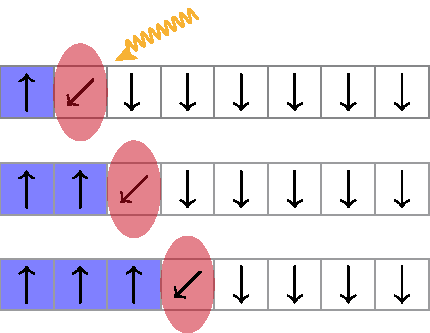
\includegraphics{figures/1D_spin_lattice.pdf}
  \end{center}
  \caption{States of the 1D chain: only spins with one neighbour $\uparrow$ and the other neighbour $\downarrow$ are on resonance.}
  \label{1D_spin_lattice}
\end{figure}

Let us now define a subset of states $S$ that exist in the spin chain Hilbert space, $\ket{n}$, which have the first $n$ spins of the chain in state $\ket{\uparrow}$ with the rest $\ket{\downarrow}$. If the rule we just derived holds exactly, these states define a closed subspace. We may then write a very simple isolated Hamiltonian for this subspace:
\begin{equation}
  {\cal H}_S = \Omega \sum_{n=1}^\infty \ket{n}\bra{ n+1}+\ket{n+1}\bra{ n}.
  \label{1d_ham}
\end{equation}
The Hamiltonian couples states with $n$ up-spins to those with $n-1$ and $n+1$, with coupling strength $\Omega$. 

\section{Extension to 2D Model}

With this simplification of the 1D Hamiltonian in mind, we progress now to a semi-infinite square spin lattice with nearest-neighbour ZZ interactions. For this case we have
\begin{equation} {\cal H} = \sum_{i=1}^{\infty}\sum_{j=1}^\infty
  \epsilon \sigma^{i, j}_z + J \sigma_z^{i, j}\sigma_z^{i+1, j} +
  J\sigma_z^{i, j}\sigma_z^{i, j+1} + 2 \Omega \sigma_x^{i, j}
  \cos(\omega t).
\end{equation}
By again considering the terms affecting a particular spin in the main body of the lattice ($k(>1), l(>1)$ say) we find for $\omega = \epsilon$ and after moving to a rotating frame and making the rotating wave approximation:
\begin{equation}
  {\cal H} = J \sigma_z^{k, l} (\sigma_z^{k+1, l} + \sigma_z^{k, l+1} + \sigma_z^{k-1, l} + \sigma_z^{k, l-1}) +...
\end{equation}
where we do not explicitly write out terms not involving spin $(k, l)$.  The microwave is now only resonant for spin $(k, l)$ if it has two neighbour spins in each orientation. For a spin on the edge of the lattice there are an odd number of neighbours so resonance cannot be achieved in this case. However, applying a second microwave with $\omega = \epsilon - J$ allows resonant flips on the edge if two neighbours are down and one up - and this second field has no effect on the bulk spins.

The spin to be measured is the corner spin ($i=j=1$) and so would form part of a wider computational apparatus. We may therefore assume that it is a different species with a unique resonant frequency. The dynamics of the whole lattice may then be summarised by three rules (in order of precedence):
\begin{enumerate}
  \item The corner (test) spin is fixed.\vspace{-0.2cm}
  \item An edge spin can flip if it has one of its neighbours up and
    two down.\vspace{-0.2cm}
  \item A body spin can flip if it has two of its neighbours up and two down.\vspace{-0.2cm}
\end{enumerate}
We begin by supposing all spins are initialised in the `down' state apart from the test spin, which is located in the upper left hand corner of our lattice. We can describe this initial state by choosing two basis elements: $\ket 0$ when the test spin is down, and $\ket 1$ when the test spin is up. Using our heuristic rules we can see that these two states do not couple to each other - that $\bra 0H\ket 1=0$. In fact $\ket 0$ does not couple to any other state, so if we start in the $\ket 0$ state no amplification occurs, as desired.


\section{Building a Subspace Basis} 

We will now seek to construct a basis for the subspace containing our system evolution, by looking at states connected by our Hamiltonian. It will be convenient to represent these states on the nodes of a graph, using the edges to represent non-zero elements of the Hamiltonian.

Our starting point is the state $\ket 1$, with just the corner spin `up'. From this position our rules allow two possibilities: either the spin to the right of the corner flips, or the spin below it flips (see Fig.~\ref{partition_states}). In each case, the magnitude of the transition matrix element is $\Omega$. As we continue this procedure, we notice that the states that arise for each excitation number can be characterised by a non-increasing sequence of integers that represent the number of `up'-spins in each column of the lattice (see Fig.~\ref{partition_states}). Such sequences can also be used to define partitions of at integer: ways of splitting an integer up into a sum of other integers, e.g. $3=3=2+1=1+1+1$. In fact, the states that arise are in 1-to-1 correspondence with such partitions; we call these states `partition states' and denote them with standard partition notation (see Fig.~\ref{partition_states}).
\begin{figure}
  \begin{center}
    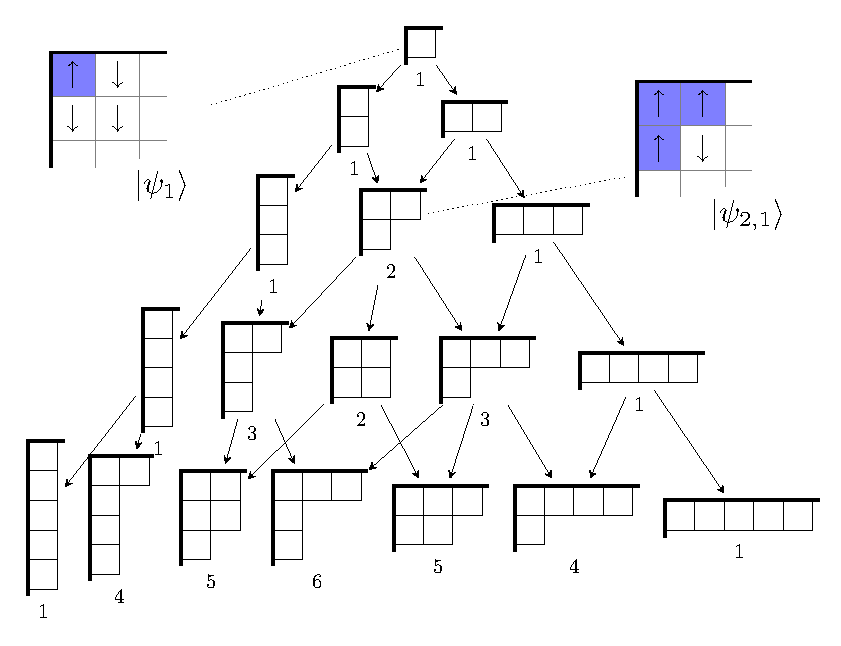
\includegraphics[scale=0.8]{assets/youngs_lattice_with_spins}
  \end{center}
  \caption{Partition states arranged into a lattice. Edges represent a coupling
    through the Hamiltion of strength $\Omega$. Weights represent the
  number of different paths through the lattice to a given state.}
  \label{partition_states}
\end{figure}
The graph we have just described is depicted in Fig.~\ref{partition_states}  is known as `Young's lattice' and arises in areas of pure mathematics, such as the representation theory of the symmetric group, and the theory of differential posets \cite{Sagan:2001p6568}. We have drawn weights beneath each state, recording the number of ways the state can be constructed. We will now further reduce the dimension of this basis
by eliminating combinations of states which are inaccessible.

Starting with $\ket 1$ we see that $\bra 1H\left(\alpha_{1,1}\ket{\psi_{1,1}}+ \alpha_{2}\ket{\psi_{2}}\right) =\Omega\left(\alpha_{1,1}+ \alpha_{2}\right)$ so $\ket 1$ does not couple to the two-excitation state $\ket{\psi_{1,1}}-\ket{\psi_{2}}$. We can eliminate this, leaving a single orthogonal, coupled state with two excitations: $\ket 2 := \frac{1}{\sqrt{2}}\left( \ket{\psi_{1,1}}+\ket{\psi_2} \right)$.

We may continue to build up coupled states with larger excitation numbers, and in fact we find that there is only a single coupled state in each case (i.e. we can always eliminate $k-1$ combinations of partition states with $k$ excitations).  To see this, first suppose we have the coupled state with $k$ excitations, which by analogy with the 1D case we write as $\ket k$. We can write $\ket k=\frac{1}{N_k}\sum_{i\in P(k)}c_{i}\ket{\psi_{i}}$, where $P(k)$ is the set of partitions of the integer $k$ and $N_k$ a normalisation factor. We want to construct the state $\ket{k+1}$ by eliminating the $k$-dimensional subspace with $k+1$ excitations, to which $\ket{k}$ does not couple.

Let $\ket{\psi}=\sum_{j\in P(k+1)}\alpha_{j}\ket{\psi_{j}}$ and consider the states $\ket{\psi}$ such that \[ 0=\bra kH\ket{\psi}=\sum_{i\in P(k)}\sum_{j\in P(k+1)}c_{i}^{*}\alpha_{j}\bra{\psi_{i}}H\ket{\psi_{j}}\] but $\bra{\psi_{i}}H\ket{\psi_{j}}=\Omega$ if $i$ is a {\it parent} of $j$ (a state connect to $j$, in the lattice row above it), and $0$ otherwise, so \[0=\bra kH\ket{\psi}=\sum_{j\in P(k+1)}\alpha_{j}\sum_{i\in parents(j)}c_{i}^{*}.\] This is the equation of a hyperplane in $|P(k+1)|$ dimensions, defining the states that are not coupled to $\ket k$ through the Hamiltonian.  There is a unique single state orthogonal to this hyperplane, $\beta_{j}=\sum_{i\in parents(j)}c_{i}$, to which $\ket k$ couples.  So the only state with $k+1$ `up'-spins that $\ket k$ couples has coefficients proportional to $\beta_{j}$. After normalisation, we call this state $\ket{k+1}$.

Unfortunately there is no easy way to write down the partition states and weights for the $n$th row of the lattice. Fortunately, for our purposes, we only need to know that the states $\ket k$ exist and what the coupling between them is. To find this coupling, consider
\begin{align}
  g_{n-1,n} & = \bra nH\ket{n-1} \nonumber\\
  & = \frac{1}{N_{n-1}N_n}\sum_{i\in P(n)}\sum_{j\in
  P(n-1)}c_{i}^{*}c_{j}\bra{\psi_{i}}H\ket{\psi_{j}} \nonumber\\
  & = \frac{1}{N_{n-1}N_n}\Omega\sum_{i\in P(n)}c_{i}^{*}\sum_{j\in
  parents(i)}c_{j} \nonumber\\
  & = \frac{1}{N_{n-1}N_n}\Omega\sum_{i\in P(n)}|c_{i}|^{2} =
  \Omega\frac{ N_n}{N_{n-1}}\label{coupling_as_sum_c2}\end{align}
To find the $N_n$ we need the sum of the squares of the weights of partitions in a given row. A standard result about Young's lattice immediately gives us this sum: $n!$ \cite{STANLEY:1975p6605}.

This result can be taken straight from the representation theory of the symmetric group: it can be shown that the nodes and their weights represent the irreducible representations and their dimensions. Given that the dimension of each representation is its multiplicity in the regular representation (with dimension $|S_n| = n!$), by dimension counting the result follows. However, for our purposes it is more enlightening to focus on a differetial poset approach, which uses particular combinatorial features of the lattice to produce the result. Here we give a brief overview of the approach detailed by Sagan in \cite{Sagan:2001p6568}.

Let $L$ be an operator that takes a partition state to a sum of its
children, and $R$ take a state to the sum of its parents. For example\begin{eqnarray*}
  L\ket{\psi_{1}} & = & \ket{\psi_{1,1}}+\ket{\psi_{2}}\\
  R\ket{\psi_{2,1}} & = & \ket{\psi_{1,1}}+\ket{\psi_{2}}\end{eqnarray*}
We add a state $\ket\emptyset$ such that $L\ket\emptyset=\ket{\psi_{1}}$
and $R\ket\emptyset=0$. Then
\begin{align}
  L^{n}\ket\emptyset=\sum_{i\in P(n)}c_{i}\ket{\psi_{i}}
\end{align}
and
\begin{align}
  R^{n}L^{n}\ket\emptyset=\sum_{i\in P(n)}|c_{i}|^{2}
\end{align}
We then need to use two facts about the structure of the lattice: that each element has one more child than it does parents, and each pair of elements either share both a single parent and a single child, or neither. The first of these properties is easy to see: each child corresponds to adding a square at a concave corner of the diagram, and each parent corresponds to removing a convex corner. These corners alternate along the boundary of the shape, starting and ending with concave ones, and so there is always one more child than parents.  The second property requires more work, but is roughly because two elements share a parent if, when placed on top of one another they differ by precisely two squares. Taking the union of these shapes you can find the unique child that they also both share.

These properties imply the commutation relation $RL-LR=I$, so
\begin{align}
  R^{n}L^{n}\ket\emptyset=R^{n-1}L^{n}R\ket\emptyset+nR^{n-1}L^{n-1}\ket\emptyset=...=n!\ket\emptyset
\end{align}
and so, $n!=\sum_{i\in P(n)}|c_{i}|^{2}$.

Referring back to Eq. (\ref{coupling_as_sum_c2}), and using $N_i=\sqrt{i!}$, we see that
\begin{equation}
  {\cal{H}} = \Omega \sum_{n} \sqrt{n} \left( \ket{n-1} \bra{n} +
  \ket{n} \bra{n-1} \right) .
  \label{2d_ham}
\end{equation}
In essence we have established a linear sequence of states, each coupled to the next analogously to the states on a 1D chain \ref{1d_ham}. However, each of our states is in fact a superposition of many configurations of the 2D array, and crucially the effective coupling from each state to the next increases along the sequence.

\section{Rate of Spin Propagation}

It has been shown (e.g. \cite{Fitzsimons:2005p6472}) that a quantum state released at the end of a semi-infinite chain of states, with constant couplings, will travel ballistically: the average position of the state along the chain is proportional to the time passed, and inversely proportional to the coupling strength. Since, in the one-dimensional case, the position is proportional to the number of spins that have flipped, we have that the total polarisation will increase linearly with time.

We can establish the rate of propagation in the 2D case using the ansatz that the time taken to travel between two neighbouring nodes is inversely proportional to the strength of the coupling between them. The total time is then $t_{2D}\propto \sum_{i=1}^{n}\frac{1}{\sqrt{i}}\simeq n^{\frac{1}{2}}$. As in the one-dimensional case, the position along the chain corresponds to the  number of spins that have flipped, and so we would expect the total polarisation to be proportional to $t^2$. This prediction of a quadratic speed-up of signal going from 1D to 2D is the central result of the chapter, and was confirmed by simple numerical simulations of Eq.~(\ref{2d_ham}) (Fig. \ref{comparison}).

\begin{figure}
  \begin{center}
    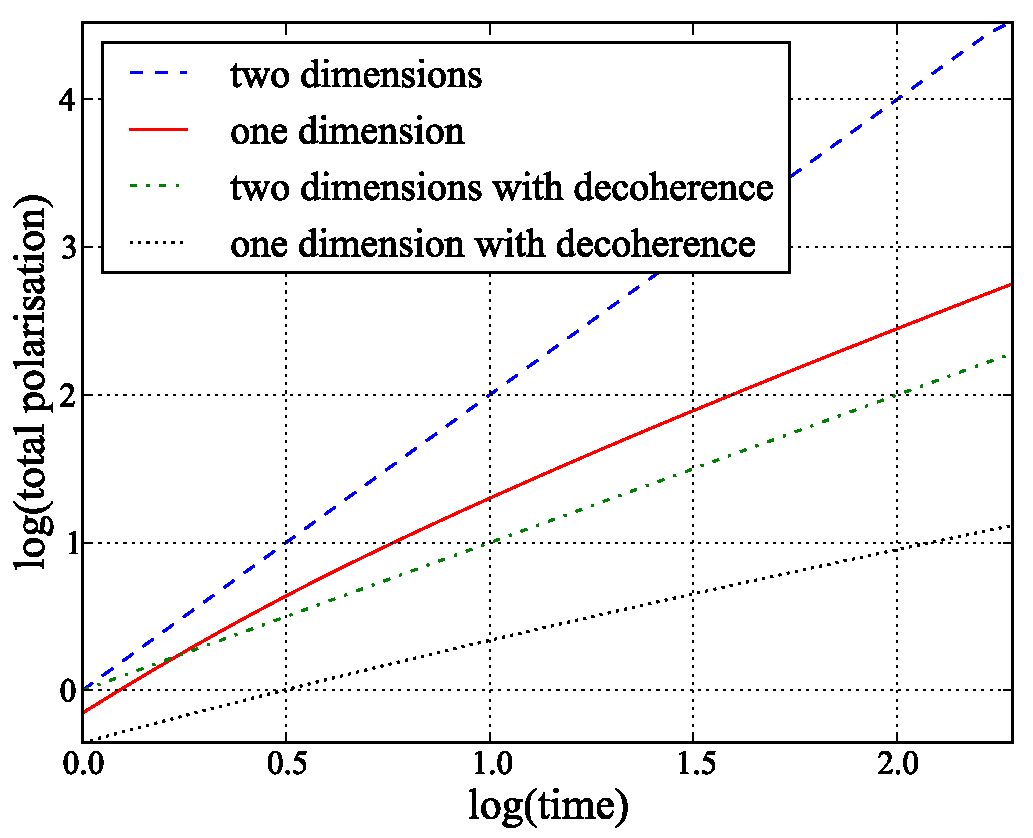
\includegraphics[scale=0.7]{assets/comparison.pdf}
  \end{center}
  \caption{Expected total polarisation against time. Time in units of $\frac{1}{\Omega}$, dephasing rate $\Gamma = 1$. The gradient of the `one dimension with decoherence' line tends to $\frac{1}{2}$ asymptotically.}
  \label{comparison}
\end{figure}

\section{Extension to 3D}

Unfortunately the mapping from 2D to 1D is not readily extendible to 3D. However, our results so far could have been anticipated using simple dimensional arguments; if one postulates that the rate of spin propagation is proportional to the boundary of the region, one can predict the correct scaling behaviour. In 1D the boundary size is independent of the region size; no matter how many spins have flipped, it still has size one. The coupling strength between states $\ket{n}$ is constant. In the 2D case, the boundary size scales with the square root of the area, and the coupling goes with $\sqrt{n}$. In 3D, the boundary scales like the cube root of the volume squared, and so we expect the coupling to scale as $n^{\frac{2}{3}}$. Following similar logic to that used in 2D case: $t_{3D}\propto \sum_{i=1}^{n}\frac{1}{i^\frac{2}{3}}\simeq n^{\frac{1}{3}}$, and so $n \sim t^3$.  


\section{Robustness against Decoherence}

We now consider the effect of decoherence. Much of the early work on continuous time quantum random walks looked at the speedup they afforded over their classical counterparts~\cite{Farhi:1998p6471}, but didn't make  any statement about the conditions under which we would expect the quantum walk to exhibit classical behaviour, as we might expect in a regime of suitably heavy dephasing, say.

We begin by considering a collective noise operator: $ L=\sum_{n}n\ket n\bra n$.  This represents noise that applies uniformly to the whole lattice: global fluctuations in the magnetic field, for example. As the effect of this type of noise depends only on the number of `up' spins, the system remains in the reduced basis of number states calculated earlier, with only the coherences between these states affected.

Our starting point is the Lindblad master equation
\begin{equation}
  \dot{\rho}=i\left[\rho,H\right]+\frac{1}{2}\Gamma\left(2L\rho
  L^{\dagger}-L^{\dagger}L\rho-\rho L^{\dagger}L\right).
\end{equation}
We proceed by splitting up the equation into diagonal and off-diagonal terms
\begin{align}
  \dot{\rho}_{ii} & = i\sum_{k=\pm i}\left(\rho_{ik}g_{ki}-\rho_{ki}g_{ik}\right)=-2\sum_{k=\pm i}Re\left[\rho_{ik}g_{ki}\right] \label{rhoii}\\
  \dot{\rho_{ij}} & = i\left(\sum_{k=\pm j}\rho_{ik}g_{kj}-\sum_{k=\pm i}\rho_{kj}g_{ik}\right)-\Gamma\rho_{ij}
\end{align}
where $g_{ij}$ is the coupling between states $i$ and $j$. In the limit of heavy dephasing ($\Gamma\gg g$), we have a process similar to adiabatic following, and we can make the approximation\[ \Gamma\rho_{ij}\approx i\left(\sum_{k=\pm j}\rho_{ik}g_{kj}-\sum_{k=\pm i}\rho_{kj}g_{ik}\right).\] We consider the $\rho_{ij}$ as a set of $\frac{n(n-1)}{2}$ variables and solve for them in terms of the $\rho_{ii}$. Neglecting terms that are second order in $\frac{g}{\Gamma}$, and substituting back into Eq. (\ref{rhoii}) gives \[ \dot{\rho}_{ii}=-\sum_{j=i\pm1}\frac{2|g_{ij}|^{2}}{\Gamma}\left(\rho_{ii}-\rho_{jj}\right).\]
Our quantum chain formally reduces to a classical Markov chain on the same statespace, with transition rates proportional to the coupling squared. 

In one-dimension $g_{ij} = 1$ and we are reduced to a simple random walk on a semi-infinite line. By analogy with simple diffusion we expect that the resulting distribution is roughly Gaussian, with the expected number of flipped spins going with $\sqrt{t}$: the rate of spin propagation drops from $t$ to $\sqrt{t}$. This result was confirmed numerically - although (Fig. \ref{comparison}) appears to show something closer to a $t^\frac{2}{3}$ dependence, (Fig.~\ref{asymptotic_1d}) shows that the $\sqrt{t}$ value is recovered as time increases.

\begin{figure}
  \begin{center}
    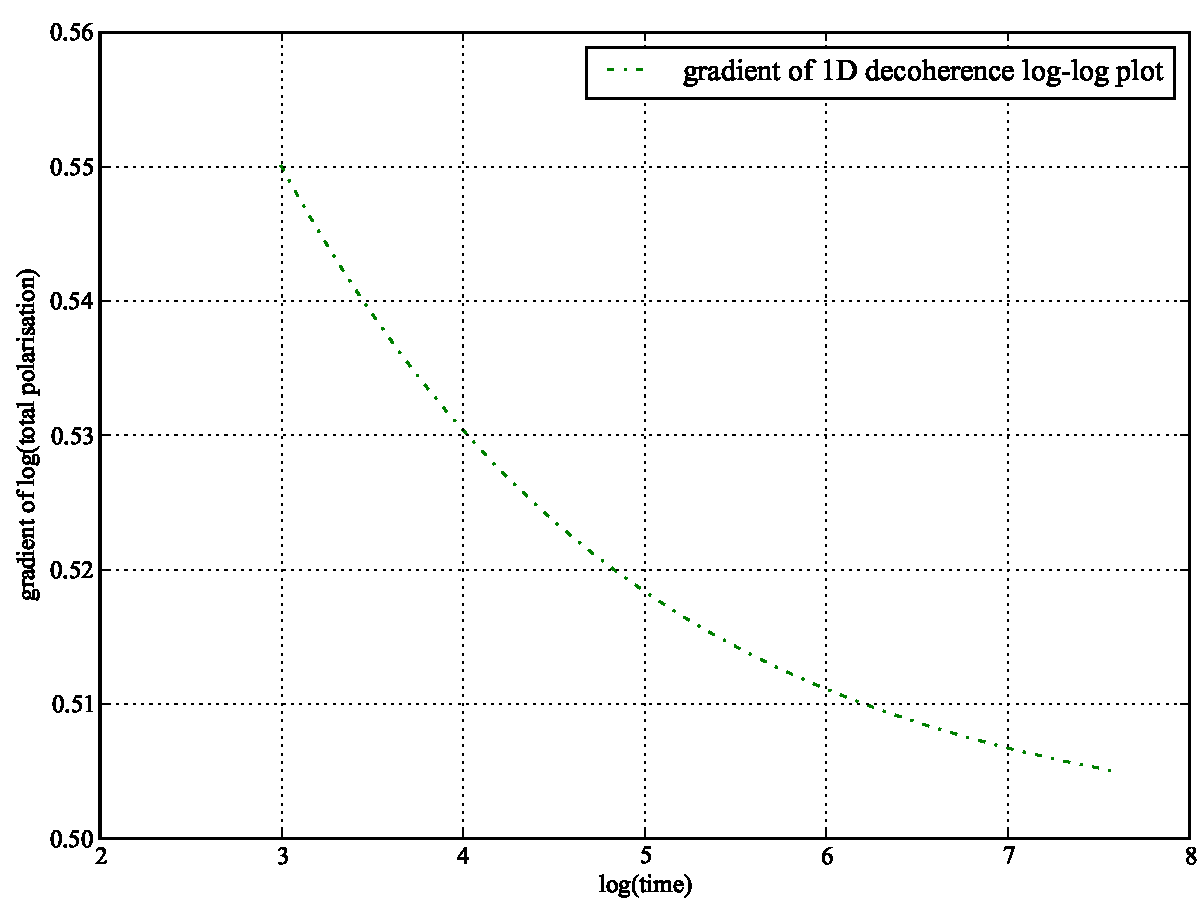
\includegraphics{assets/asymptotic_1d.pdf}
  \end{center}
  \caption{ The gradient of the `one dimension with decoherence' line tends to $\frac{1}{2}$ asymptotically.}
  \label{asymptotic_1d}
\end{figure}

In the two-dimensional case $g_{ij} = \sqrt{j}, j=i+1$: We get a random walk with increasing transition rates. Numerically (Fig. \ref{comparison}), we find that the rate of spin propagation drops from $t^2$ to $t$ - still an encouraging scaling.

        %%\subsection{Independent noise}

So far we considered a collective noise scenario, using a single Lindblad operator, $ L=\sum_{n}n\ket n\bra n$ . This is convenient to analyse for our system, as the system remains in the subspace covered by our basis of number states. A more realistic model involves treating the noise occurring at each site as independent. In this case we have Lindblad operators of the form
\begin{equation}
  L_i = \sigma_z^i
\end{equation}
for lattice sites $i$. Following a similar procedure to before we find the equivalent classical chain to be
\begin{equation}
  \dot{\rho}_{ii}=-\sum_{j\in
  P(i)}\frac{2|g_{ij}|^{2}}{\Gamma}\left(\rho_{ii}-\rho_{jj}\right)
  \label{qmat}
\end{equation}
where, crucially, the index now runs over all the partition states, rather than our basis of accessible states. In fact, in the 1D case these states are one and the same, and so the spin propagation goes as $\sqrt{t}$, as found in the collective noise case. In the 2D case, we are now performing a continuous-time classical random walk on Young's lattice. We are able to use the property that each node always has one more child than parents, to predict that the rate of spin propagation will be proportional to $t$ - the same as the collective noise case.  

\begin{figure}
  \begin{center}
    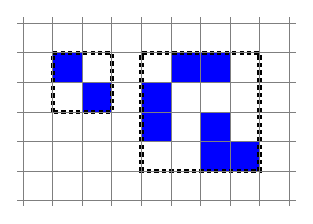
\includegraphics[scale=1]{assets/impurity}
  \end{center}
  \caption{Maximum extent of propagation of initialisation
    imperfections in the lattice - due to propagation rules
  imperfections are unable to grow beyond the dotted bounding boxes. }
  \label{impurities}
\end{figure}


\section{Robustness against Imperfect Initialisation}

Finally we consider imperfect inital polarisation (i.e. finite temperature) - a property exhibited by any real experimental system.  
A fortuitous consequence of the propagation rules is that our system is particularly robust against this source of error; it is difficult for imperfections in the centre of the lattice to spread (Fig. \ref{impurities}).

To estimate an upper bound for our initialisation threshold we took a randomly initialised lattice, with given imperfection probability, and evolved it using purely deterministic rules, to see whether the imperfections grew to cover over half the lattice. We expect this to give a loose upper bound for the quantum case, as quantum imperfections will both grow and shrink, making it less likely that they will compound in the same manner as deterministic growth. Fig \ref{flipthreshold} shows the results of these simulations; below $4\%$ the probability of growing to cover the majority of the lattice is negligible.
\begin{figure}[!h]
  \begin{center}
    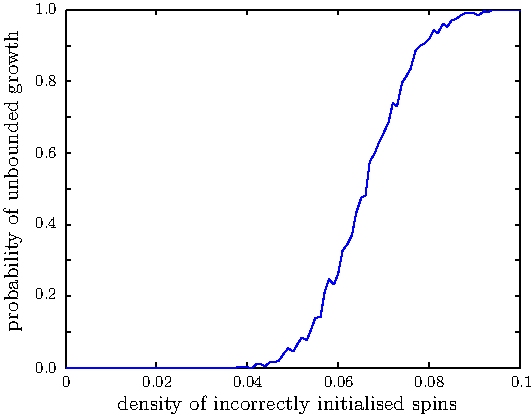
\includegraphics{assets/flipthreshold.pdf}
  \end{center}
  \caption{Probability that imperfections at given density will deterministically grow to cover over half the lattice.}
  \label{flipthreshold}
\end{figure}

This threshold places our protocol well within experimental capabilities; for example for an array placed in a standard W-band electron spin resonance system ($100$ GHz) and cooled using liquid 4He to $1.4$ degrees Kelvin, only $3.1\%$ of electron spins will be in the `up' state.

%\begin{acknowledgements}
%we thank gerard milburn and john morton for useful discussion. this work was supported by the epsrc, the national research foundation and ministry of education, singapore, and the royal society.
%\end{acknowledgements}
%\section{Conclusion}

%Although we know how the expected number of flipped spins increases with time, we have so far said nothing about how these spins are distributed throughout our sample. To investigate this we have plotted the value of the expected flipped spin density over the course of the evolution.  
%\begin{figure}[ht]
%  \begin{center}
%    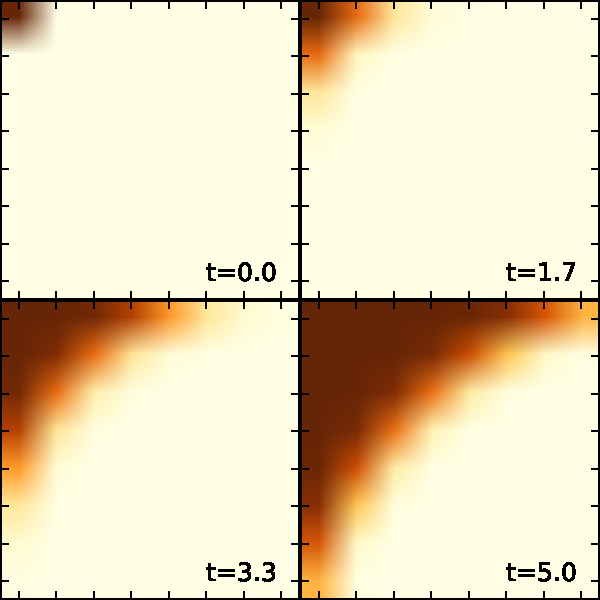
\includegraphics[scale =0.8] {assets/density_fig_all.pdf}
%  \end{center}
%  \caption{Density of flipped spins with time}
%  \label{densitypics}
%\end{figure}

%As you can see (Fig. \ref{densitypics} ), the area of high density is triangular in shape, of dimensions that scale linearly with the time elapsed. The boundary between areas of high and low density remains remarkably sharp, considering that the number state basis elements on which the motion is based have diffuse boundaries themselves.



\section{Conclusion and Further Work}

Electron and nuclear spins have been employed in many of the early demonstrations of quantum technology but applications in real world QT are limited by the difficulty of measuring single spins. In this chapter we have shown that it is possible to rapidly and robustly amplify a spin state using a lattice of ancillary spins. The model we have employed corresponds to an extremely simple experimental system: a homogenous Ising-coupled spin lattice in one, two or three dimensions, driven by a continuous microwave field. We have constructed a natural basis for the problem and used this to assess the rate of amplification, both ideally and in the presence of environmental noise. We establish that the process can operate at finite temperature (imperfect initial polarisation) and under the effects of various forms of decoherence.

There are several directions in which the work presented in this paper could be extended. As noted, our strategy for the construction of the Hamiltonian for the reduced system does not transfer directly into the 3D case. It could be that further study of the system would yield a closed form, which would allow us to verify our claims about the rate of spin propagation in a 3D system.

There is also potential to develop the ideas discussed here to provide an experimental test for the regularity of a lattice structure: the ability to perform a controlled expansion, and later contraction, of the lattice polarisation would provide evidence of a uniform structure. Further theoretical work could focus on characterising the possible signatures of semi-regular array structures.




\chapter{A Reliable, Efficient Source for Indistinguishable Photons} 
\label{ch:SinglePhotonSource}

\section{Introduction}
% [ Use of single photon sources ]

Single photon sources are an essential component of many quantum information processing (QIP) protocols, from quantum key distribution (QKD) protocols \cite{bennett_brassard_84, ekert_91} to linear optical quantum computing (LOQC) schemes \cite{knill:2001, kok07, kok10}.
As described in Section \ref{remote_entanglement_generation}, optical schemes using path erasure  can be used to generate long-range entanglement between physically separated systems  \cite{barrett+kok, bose99, simon:03, lim05}. Such procedures can be repeated on many different pairs of systems and so create a distributed cluster state~\cite{raussendorf01,kok10}, which is the key resource required for implementation of measurement based quantum computing (Section \ref{MBQC}).

In order to be useful in these applications, a photon source must be of a high quality in two respects: it must reliably produce a single photon on demand, and the photons produced must be indistinguishable from one another. 

To be perfectly indistinguishable, photons must have the same pulse width, band width, polarization, arrival time at the detector, and carrier frequency. Indistinguishability is vital if photons are to exhibit high quality quantum interference, and its consideration is therefore critical when designing photon sources for LOQC and path erasure entanglement generation.
If photons can be distinguished even in principle, this can lead directly to imperfect LOQC gates, or to a lessening of the degree of entanglement generated in distributed cluster states. In QKD, indistinguishability is less important as interference effects are not required, but it is of paramount importance that no more than one photon is emitted on demand; multiple photon emission leads to security loopholes~\cite{kok10}.

As a measure of indistinguishability we exploit the Hong-Ou-Mandel (HOM) effect \cite{HOM}, which relies on the bunching behaviour of identical photons when they are incident on a beam splitter with the same temporal profile. As explained in Section \ref{HOM_section}, if the photons are indistinguishable, they will always emerge in and be detected in the same output arm (Fig.~\ref{HOM_expt}). The number of same-arm detection events are usually plotted as a function of arrival time of the two photons - and hence a `dip' at a time difference of zero is an indicator of indistinguishability.
\begin{figure}[htb]
  \begin{center}
  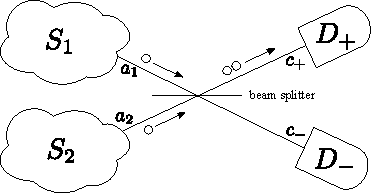
\includegraphics[width=8cm]{assets/HOM_expt.pdf}
  \end{center}
  \caption{Hong-Ou-Mandel effect: a pair of photons from two sources $S_1$ and $S_2$ incident on a beam splitter exhibit perfect bunching behaviour if they are completely indistinguishable. In this case the detectors  $D_+$ and $D_-$ will never click simulataneously.}
  \label{HOM_expt}
\end{figure}
The degree of distinguishability can be given by the Hong-Ou-Mandel visibility, $v_{\rm HOM}$, which is the proportion of same-arm detections, over many runs of the experiment. It is worth noting that this definition of $v_{\rm HOM}$ differs from the Hong-Ou-Mandel dip commonly measured in experiments: the typical experimental setup involves continuously pumped systems, and looks for an absence of simultaneous detections in different detector arms; we consider an on-demand photon pair, and look at the probability that the two detections are in the same arm \textit{over the complete run of the experiment}. 

As mentioned above, besides indistinguishability an essential characteristic of a good photon source is that it will consistently produce a single photon, but never more than one, on demand~\cite{lounis05}.  A laser source can be attenuated so that it gives zero or single photons most of the time. However, photons from classical lasers sources obey Poissonian statistics so that in order to keep the two-photon event rate low the probability of a single photon may become unworkably small for many applications. In addition to this, Poissonian sources are unsuitable for two-photon interference experiments since the rate of two photon production from a single source is similar to that for a single photon from each source~\cite{kok10}.
%In contrast, low-dimensional optically active quantum systems such as self-assembled semiconductor quantum dots \textcolor{red}{REFS} do not suffer from this problem and routinely achieve near perfect anti bunching in $g_2$  experiments  \textcolor{red}{REFS}.
It is worth noting that perfect efficiency should never be a requirement in any realistic optical QIP scheme, as these schemes must always be tolerant to photon loss within other parts of the apparatus. However, a good photon source must be reasonably efficient to be useful, and we should not be forced to trade efficiency for other desirable characteristics.

% [ Schemes that have been suggested in the past ]

The use of low-dimensional quantum systems as single photon sources avoids the efficiency problems of Poissonian sources. Successful experimental implementations have been realised in a number of different systems including atom-cavity schemes \cite{rempe:prl:02, kimble:sci:04, grangier:sci:05, rempe:nat-phys:07}, quantum dots \cite{arakawa:nat-mat:06, imamoglu:nat:07} and diamond colour centres \cite{roch:njp:07, bernien:prl:12, lukin:prl:12}. While the majority of the work has been focussed on the efficient production of a single photon, recent experiments in NV centres \cite{bernien:prl:12, lukin:prl:12} and quantum dots~\cite{flagg10, patel10} have demonstrated two-photon interference effects from different sources, albeit sacrificing efficiency by filitering out undesired frequencies. It has been suggested that cavities could be used in these systems, to enhance the emission into the target mode, reducing the need for filtering \cite{greentree:08}.

In order to improve the characteristics of a photon source, it is not sufficient to simply consider the material parameters of the system being used: one should also consider the approach used to control the system. Perhaps the simplest strategy is to excite the system first optically, either coherently or incoherently, and wait for the system to relax into its ground state, emitting a photon in the process; we will henceforth refer to this as the `pulse-relax' technique. % focussing on coherent exitation. 
This approach makes minimal resource demands on the system and, due to its simplicity, is the technique proposed in some remote entanglement generation schemes~\cite{barrett+kok,simon:03}. The pulse-relax approach is problematic in systems where the excited state is sensitive to decoherence, which will degrade the photon's indistinguishability \cite{kiraz:2004, santori:2009, barrett+kok, nazir09}. These effects can be reduced, for example by exploiting the Purcell effect to enhance the emission rate into the desired photon mode~\cite{purcell46,englund05} or by using temporal post-selection of emitted photons~\cite{nazir09}. However with experimental limits on cavity couplings both of these inevitably lead to lower efficiency as the proportion of emissions that are utilized falls \cite{auffeves:prb:10}.

A fundamentally different approach is to use more elaborate QED schemes to release a photon from the system in a controlled manner. In particular single photon sources using a Raman approach have been analysed \cite{kiraz:2004, santori:2009} and experimentally realised \cite{rempe:prl:02}. The approach places more demands on the system, requiring a  three level system with a $\Lambda$-system configuration.
\begin{figure}[htb]
  \begin{center}
  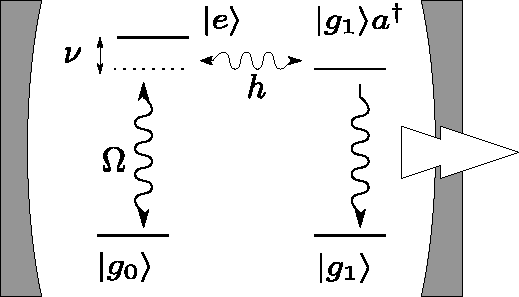
\includegraphics[width=8cm]{assets/lambda_system.pdf}
  \end{center}
  \caption{Effective level structure of a driven $\Lambda-$system inside an optical cavity. Here, $\Omega$ is the amplitude of an external (laser) driving field, $h$ the optical dipole-cavity-coupling, and $\nu$ the shared detuning of the laser and the cavity transition frequency  from the excited state. The system can decay into state $\ket{g_1}$ and in doing so emit a photon into a well-defined external mode.}
  \label{lambda_system}
\end{figure}
Each arm is coupled to either a classical or a quantum light field; in Fig~\ref{lambda_system} we show the situation when one arm is driven classically, with a coupling $\Omega$, and the other arm is coupled to a cavity mode with strength $h$. By detuning both arms of the $\Lambda$-system by the same amount $\nu$, population is transferred from one arm to the other, whilst suppressing population in the top state. Provided that the coupling strengths are small in comparison to the detuning, $\Omega \ll \nu$ and $h\ll\nu$, we induce an effective coupling between the two low-lying states, which causes oscillations with Rabi frequency ${h\Omega}/{4 \nu}$. The population in the excited state remains small at all times, and so any decoherence that arises due to environmental coupling to this excited state may be reduced using this strategy. In particular, a common realisation of a single photon source is a quantum dot, in which the excited state typically has a different charge configuration to the ground state. This causes local lattice distortions, which in turn locally alter the electronic bandgap, thus inducing a coupling to acoustic phonons~\cite{ramsay:2010, mahan00} that can act as a noise source. 
% [ Overview of what we will do ]

In this chapter we provide a detailed and realistic analysis of the effects of the lattice vibrations for single photon emitters based on (self-assembled) semiconductor quantum dots. By comparing a standard pulse-relax approach with the aforementioned Raman technique, we find that the latter can can offer considerable improvements in terms of both photon indistinguishability and source efficiency. Our results extend and complement a previous study \cite{santori:2009} which considered generic pure dephasing noise. However, here we also show that the precise choice of control parameters is important if phonon-induced decoherence is to be successfully suppressed.

\section{Our model}

% [ The basic setup ]

For convenience of notation we consider the $\Lambda$-system detailed in Fig.~\ref{lambda_system} for both the pulse-relax and the Raman approach. 
%In the former case we are only interested in the transition from one of ground states to the common excited state. 
In both cases one arm of the system is coupled to the cavity with detuning $\nu$. % where we denote the frequency mismatch between cavity and $\Lambda$-system transition by $\nu$. 
In the Raman scheme, the other arm is driven with strength $\Omega$ by a laser with a matching detuning $\nu$, and the system starts in state $\ket{g_0}$. By contrast, we model the pulse-relax approach by setting $\Omega = \nu = 0$ and starting in state $\ket{e}$, ignoring the details of the excitation process. The fact that we are neglecting the excitation step in this simplified picture will slightly favour the pulse-relax approach in terms of production rate, but is largely justified on the assumption that the initial excitation process takes place quickly compared with other system dynamics. Our framework thus allows us to consider the pulse-relax approach as a special case of the master equation we will now derive for the Raman approach.

We split the Hamiltonian into contributions from the emitter system and cavity ($sys$), the driving laser ($dr$), the unperturbed phonon bath ($ph$) and interaction terms between the system and phonon bath ($sys-ph$), system and target external mode ($sys-mod$), and system and other external modes ($sys-ext$):
\begin{eqnarray}
  H = H_{sys} + H_{dr} + H_{ph} + H_{sys-ph} + H_{sys-mod} + H_{sys-ext}~.
\end{eqnarray}
The $H_{sys-mod}$ and $H_{sys-ext}$ terms are well understood, and we will treat these by adding in the appropriate Lindblad terms to our final master equation. In the following, we shall describe the rest of these terms separately. 

Using the standard Jaynes-Cummings Hamiltonian (Section \ref{JC_Ham}), the $\Lambda$-system coupled to a cavity mode with strength $h$ and detuning $\nu$ from resonance  can be described by the following Hamiltonian:
\begin{eqnarray}
  H_{sys} = \left(\omega + \nu\right)\ketbra{e}{e} + \omega a^\dagger a + \frac{h}{2}\left(\ketbra{g_1}{e}a^\dagger + \eqntext{h.c.} \right)~,
\end{eqnarray}
where $\eqntext{h.c.}$ denotes the Hermitian conjugate. $\omega$ is the cavity mode frequency.

We can restrict ourselves to one or zero cavity photons since the Jaynes-Cummings model preserves excitation number and after photon emission we assume that the emitter system remains in state $\ket{g_1}$ - i.e.\ we make the approximation that once a photon has escaped re-excitation does not occur - at least until an appropriate reset step (such as thermal relaxation) which we assume happens on a much longer timescale than the photon emission dynamics. This allows us to replace $\ket{g_1}a^\dagger$ with a new combined atom-photon state $\ket{g_a}$ and $a^\dagger a$ with $\ketbra{g_a}{g_a}$. 

The term $H_{dr}$ describes a laser driving the transition $\ket{g_0} \leftrightarrow \ket{e}$ with coupling strength $\Omega$, and whose frequency is detuned from resonance by the same $\nu$ parameter, yielding
\begin{eqnarray}
  H_{dr} = \Omega \cos(\omega t) \left(\ketbra{e}{g_0} + \eqntext{h.c.} \right)~.
\end{eqnarray}
After performing the rotating wave approximation, assuming that $\omega \gg \nu, h, \Omega$, we are left with 
\begin{eqnarray}
  H_{sys} + H_{dr} =  \nu\ketbra{e}{e} + \frac{1}{2}\left(h \ketbra{g_a}{e} + \Omega \ketbra{e}{g_0}\right) + \eqntext{h.c.}
\end{eqnarray}
for the total system Hamiltonian.

We model the phonons as a bath of harmonic oscillators with creation and annihilation operators, $b_q^\dagger$ and $b_q$, as in Section \ref{phonon_me}:
\begin{eqnarray}
  H_{ph} &= \sum_q \omega_q b_q^\dagger b_q,
\end{eqnarray}
which couple to the exciton state $\ket{e}$ through the deformation coupling with coupling  constants $f_q = D|q|$ in the usual way \cite{mahan00}: 
\begin{eqnarray}
  H_{sys-ph} = \ketbra{e}{e}\sum_q f_q \left(b_q^\dagger + b_q\right).
\end{eqnarray}

The effect of the phonon bath on a driven quantum dot can be described using a Lindblad master equation \cite{gauger:2008}, where the Lindblad operators  induce phonon-assisted transitions between the dressed system eigenstates \cite{gauger:2010}. We follow the derivation from Section \ref{phonon_me}. To derive the master equation we must first diagonalise the system Hamiltonian, $H_{sys} + H_{dr}$. We find that the eigenvalues are
\begin{eqnarray}
 \lambda_0 &=& 0 \nonumber, \\
 \lambda_\pm &=& \frac{\nu \pm \sqrt{\nu^2 + \Omega^2 + h^2}}{2},
\end{eqnarray}
with corresponding eigenvectors
\begin{eqnarray}
  \ket{\psi_0} &=& n_0 \left(h\ket{g_0} - \Omega\ket{g_a}\right), \nonumber \\
  \ket{\psi_\pm} &=& n_\pm \left( \Omega\ket{g_0} + h\ket{g_a} +2\lambda_\pm \ket{e} \right).
\end{eqnarray}
$n_0$ and $n_\pm$ are appropriate normalisation factors. We now make the Born and Markov approximations which lead to the master equation \cite{breuer02} in standard Lindblad form:
\begin{eqnarray}
  \dot{\rho} &= i\left[ \rho, H \right] + D_{ph}(\rho)
\end{eqnarray}
with the phonon dissipator given by
\begin{eqnarray}
  D_{ph}(\rho)  &= J(\Lambda) \left[ \left( N(\Lambda)+1 \right)D\left[ P_\Lambda \right] \rho + N(\Lambda)D[P_\Lambda^\dagger] \rho \right] 
  \label{eqn:phonondiss}
\end{eqnarray}
where $D[L]\rho = L\rho L^\dagger - 1/2(L^\dagger L\rho + \rho L^\dagger L)$, $\Lambda = \lambda_+ - \lambda_- $, and $P_\Lambda = -\ketbra{\psi_-}{\psi_+}$. Note that the phonons only induce transitions between the two optically bright system eigenstates and do not couple to the dark $\ket{\psi_0}$. In the above equation $N(\Lambda)$ is the bosonic mode occupation number:
\begin{eqnarray}
  N(\omega) &= \frac{1}{e^{\beta \omega}-1}
\end{eqnarray}
$\beta = (k_BT)^{-1}$ and we shall be henceforth consider all systems at room temperature, $T = 298$~K. The spectral density function $J(\omega)$ represents the electron-phonon coupling weighted by the density of phonon modes~\cite{breuer02}. The quantum dot system we consider is well described by taking~\cite{gauger:2008}
\begin{eqnarray}
  J(\omega) &= \alpha \omega^3 e^{-\left(\frac{\omega}{\omega_c}\right)^2}~.
  \label{eq:specdens}
\end{eqnarray}
We take $\alpha = 0.0027$~ps$^{-1}$ and $\omega_c = 2.2$~ps$^{-1}$, values that agree well with experiments on self-assembled quantum dots~\cite{ramsay:2010, ramsay2:2010}.

We absorb the rates in \eqref{eqn:phonondiss} into the Lindblad operators to obtain following decoherence operators:
\begin{eqnarray}
  U_+ &= \sqrt{J(N+1)}\ketbra{\psi_-}{\psi_+} \\
  U_- &= \sqrt{JN}\ketbra{\psi_+}{\psi_-}
\end{eqnarray}
where we have taken $J = J(\Lambda)$ and $N = N(\Lambda)$. Note that if non-Markovian dynamics are taken into account~\cite{neilsen12} this can lead to effects on the ultra-short timescale, but these are in general much shorter than typical dynamics studied here.

As a measure of the degree of indistinguishability of the photons produced in the emission process, we consider the HOM visibility, which is the normalised probability of same arm detections obtained over many runs of the experiment,
\begin{eqnarray}
v_{\rm HOM} = \frac{p_{\rm same} - p_{\rm diff}}{p_{\rm same} + p_{\rm diff}},
\end{eqnarray}
where $p_{\rm same}  = p(D_+ \cap D_+) + p({D_- \cap D_-})$ and $p_{\rm diff}  = p(D_+ \cap D_-) + p({D_- \cap D_+})$ with $p(D_x \cap D_y)$ being the probability of obtaining a click in detector $D_y$ followed by a click in detector $D_x$.

In order to calculate $v_{\rm HOM}$ we thus need to consider photons emitted from two copies of the system $S_1$ and $S_2$, one for each input arm of the beam splitter interferometer. The joint state of the system then inhabits the space $S= S_1 \otimes S_2$ (Fig.~\ref{HOM_expt}).
We label the two cavity modes using annihilation operators $a_1$ and $a_2$. Using the input-output formalism (e.g~\cite{walls+milburn}) and neglecting incoming light, we can describe the modes outside the cavities as $a_{i, \text{out}} = \sqrt{\kappa}a_{i, \text{in}}$, where $\kappa$ is the cavity leakage rate. The modes corresponding to detection in $D_\pm$ are labelled $c_\pm$ respectively. Due to the transformation performed by the beam splitter, $c_\pm$ can be written in terms of $a_1$ and $a_2$ as follows:
\begin{eqnarray}
  c_+ &= \sqrt{\kappa} \frac{1}{\sqrt{2}}\left( a_1 + a_2 \right), \\
  c_- &= \sqrt{\kappa} \frac{1}{\sqrt{2}}\left( a_1 - a_2 \right).
\end{eqnarray}
We assume that the field in the mode outside the cavity is directly related to the field inside, neglecting the process of escape from the cavity.
The effect on the system $S= S_1 \otimes S_2$ of a detection in the plus or minus output mode is then described by the projection operators
\begin{eqnarray}
  C_\pm &= \ketbra{g_1}{g_a}\otimes\id \pm \id\otimes\ketbra{g_1}{g_a}.
\end{eqnarray}

We could now simulate many trajectories of this system and build up an estimate of $v_{\rm HOM}$ by averaging these~\cite{carmichael:92}. Instead we introduce a technique that we call the \textit{semi-quantum master equation} method, which will allow us to find $v_{\rm HOM}$ in a single run of a master equation acting on a slightly larger Hilbert space.

\section{Introducing the Semi-Quantum Master Equation Method}\label{semi_quant_me_section}

We are often interested in `observable events' in quantum systems, such as the emission of a photon. When an event is observed the system undergoes a transition due to wave function collapse. During a period when no event is observed the system evolves according to a conditional master equation, reflecting the fact if events could be observed but are not, then this also informs our knowledge of the state. In order to answer questions about the probabilities and time distributions of events or chains of events, one approach is to use a quantum jump master equation to generate individual trajectories of the system. In each time step we decide probabilistically whether an event should occur. If it does occur then the system collapses according to a quantum jump; if it does not occur then the system evolves conditioned on no jump occurring. Statistics about the quantities of interest are built up as many trajectories are created.

Here we look at a different approach to calculating the quantities relating to events that occur in such systems. Instead of simulating multiple trajectories of the system, we efficiently increase the size of the statespace to record the information of interest. This allows us to calculate the desired system properties, and their time evolution, by solving a single master equation. 

Consider a system that can exist in a number of different states. Let a movement between these states constitute an event, and assume that each kind of event happens at a given rate. Such a system is heavily reminiscent of a classical continuous time Markov chain (CTMC), which can be represented as a graph with the states as nodes and the edges events weighted by the transition rates (Fig.~\ref{markov_chain}). 
\begin{figure}[htb]
  \begin{center}
  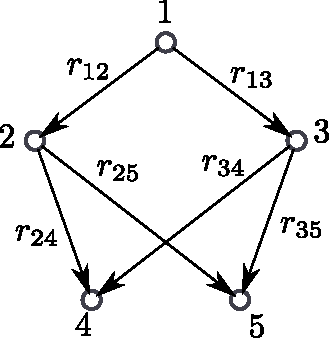
\includegraphics[]{assets/markov_chain.pdf}
  \end{center}
  \caption{A classical continuous-time Markov chain, with statespace $W = \{1,2,3,4,5\}$. The edge weight, $r_{ij}$, represents the transition rate from state $i$ to state $j$. If $\rho_i(t)$ is the population in state $i$ at time $t$, the system is governed by the rate equations $\dot{\rho_i} = \sum_{j\in W} r_{ji}\rho_j$.}
  \label{markov_chain}
\end{figure}
Given an initial state $i$ in a chain of size $n$, we can calculate the probability that at a later time $t$ the chain is in state $j$, by solving the rate equations - a set of $n$ ordinary differential equations.

Quantum systems differ from classical continuous-time Markov chains due to quantum superposition. We are not able to simply record the population in each quantum state as inter-state coherences are also important. Using a Markov chain to model the whole quantum system is not possible by definition - systems that can be modelled in this way do not exhibit quantum behaviour.

In what follows it is helpful to explain carefully what we mean by `state'. In quantum systems a state is usually a vector in the Hilbert space of the system. We shall call this a quantum-state. We can also refer to the `state' of the overall process, considering for example a system that has emitted a photon to be in a different process-state to one which has not. A system changes process-state when an event is observed.

Whereas thinking in terms of the CTMC is not useful when considering quantum-states, it is an effective way to think about process-states. As process-states are separated by an observed event, no coherences can exist between the two histories, making a CTMC approach feasible. Of course, process-states alone are not enough to model the whole system. Each process-state needs its own copy of the system attached to it. We can think of a Markov chain with a copy of our system at each node, where the transition rates are determined by the jump Lindblad operators corresponding to the events. Another way of thinking about this is that we extend our overall space with a set of process-states, to allow us to record events in the system.

Formally, we take a set of process-states $S_P$, transitions between which correspond to our observable jump events described by jump operators $J_Q^{(i)}$. We extend the Hilbert space of our quantum system $S_Q$ by forming the tensor product:
\begin{eqnarray}
  S = S_Q \otimes S_P.
\end{eqnarray}
The new Hamiltonian is given by
\begin{eqnarray}
  H = H_Q \otimes \id.
\end{eqnarray}
If event $J_Q^{(i)}$ causes a transition from system state $a$ to $b$ we say it is of type $(a, b)$. Its action on the extended system $S$ is described by
\begin{eqnarray}
J^{(i)} = J_Q^{(i)} \otimes \ketbra{b}{a}.
\end{eqnarray}
For any other Lindblad operators acting on the system $L_Q^{(i)}$, we need to create a set of size $|S_P|$ Lindblad operators - one to operate on each subspace independently:
\begin{eqnarray}
  s(L_Q^{(i)}) = \left\{ L_Q^{(i)} \otimes \ketbra{j}{j}, j \in S_P \right\}.
\end{eqnarray}

At first glance it might appear that we have increased a system of size $m = |S|$ to size $mn$, where $n = |S_P|$. Whilst this is true, the situation is not as bad as it seems at first, because the coherences between the different subsystems are unimportant -- instead of a density matrix of size $(nm)^2$ we can use a system of size $nm^2$, an increase linear in the number of system states. In practice we can often do better than this by eliminating unnecessary states from some of the subsystems.  

As a simple concrete example, consider a resonantly driven two-level system $S_Q = \{ \ket{g}, \ket{e} \}$, with Hamiltonian
\begin{eqnarray}
  H_Q = \Omega \left( \ketbra{g}{e} + \ketbra{e}{g} \right).
\end{eqnarray}
Suppose that it is also possible for the system to spontaneously emit from state $\ket{e}$ into the environment - a transition described by the jump operator
\begin{eqnarray}
  J_Q = \ketbra{g}{e}.
\end{eqnarray}

We are interested in knowing about the time distribution of the first time a photon is emitted. We add the two process-states $0$ and $1$, indicating whether the event has occurred or not. Our new system is described by:
\begin{eqnarray}
  S &=& \left\{ \ket{g0}, \ket{e0}, \ket{g1}, \ket{e1} \right\} \label{sys-start} \\
  H &=& \Omega \left( \ketbra{g0}{e0} + \ketbra{e0}{g0} + \ketbra{g1}{e1} + \ketbra{e1}{g1}  \right) \\
  J_1 &=&  \ketbra{g1}{e0} \\
  J_2 &=& \ketbra{g1}{e1}. \label{sys-end}
\end{eqnarray}
The population in the $1$ subspace at time $t$ will give us the probability a photon has been emitted by this time.

\begin{figure}[htb]
  \begin{center}
    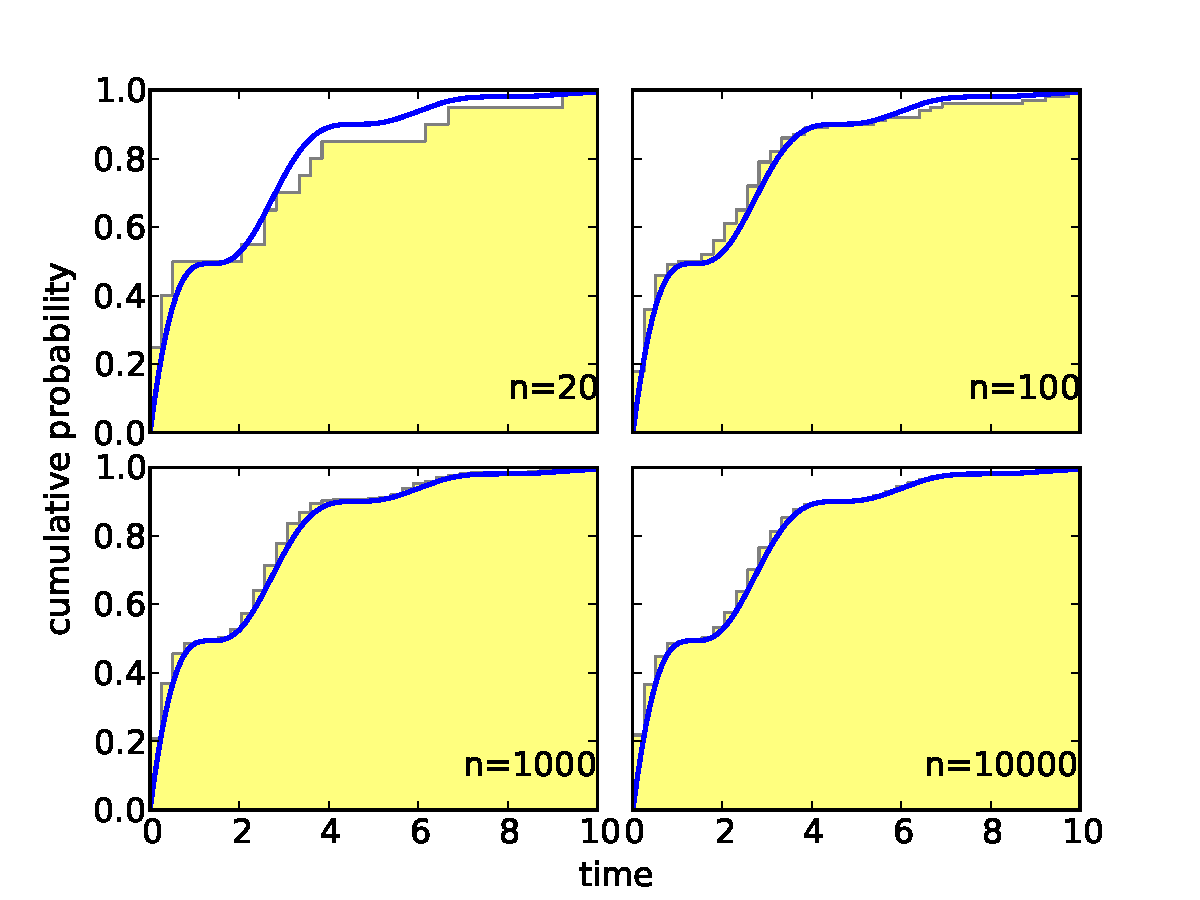
\includegraphics[width=12cm]{assets/sqme_mc_comp.pdf}
  \end{center}
  \caption{Comparison of semi-quantum master equation approach with Monte Carlo simulations of $n$=20, 100, 1000, and 10000 runs, for the system described by~\ref{sys-start}-~\ref{sys-end}. For the cumulative histogram plots we used horizontal binning with 40 bins, which explains why the horizontal resolution does not improve further for the larger values of $n$.}
  \label{sqme_mc_comp}
\end{figure}

If we only cared about this distribution, we could reduce the size of the system by replacing the states $\ket{g1}$ and $\ket{e1}$ with a single state $\ket{1}$ to keep track of the cumulative jump probability over time. We would need to remove the last two terms from the Hamiltonian as well as $J_2$, and set $J_1 =  \ketbra{1}{e0}$. Figure~\ref{sqme_mc_comp} shows the cumulative jump probability for this system, showing agreement between the SQME results and Monte Carlo simulations with increasing numbers of runs.


\section{Applying the Semi-Quantum Master Equation Method}

\begin{figure}[htb]
  \begin{center}
  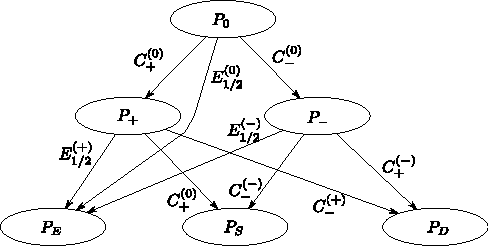
\includegraphics[width=12cm]{assets/subspace_partition.pdf}
\end{center}
  \caption{The system jump-space: On the first jump the system moves to $P_+ / P_-$ depending on the arm in which the photon is detected. After the second jump the system moves to state $P_S / P_D$ depending on whether the second photon was detected in the same or different arm to the first. At any point the system can undesirably spontaneously emit into the environment, moving to the junk state $P_E$.}
  \label{subspace_partition}
\end{figure}

When calculating $v_{\rm HOM}$ we must consider events in which photons trigger either detector, and events in which photons are spontaneously emitted into the environment. We introduce a set of process-states to record and labels these event classes (Fig.~\ref{subspace_partition}):
\begin{eqnarray}
  S_P = \left\{ P_0, P_+, P_-, P_S, P_D, P_E \right\}.
\end{eqnarray}
The process-state starts as $P_0$ and remains there until an event of interest occurs. $P_{+/-}$ represents the process-state after a single photon has been detected in the $D_{+/-}$ detectors respectively. After a second photon has been detected the process-state becomes $P_{S/D}$ depending on whether the second photon was detected in the same or different detector as the first. If at any point a photon is emitted into the environment the process moves to state $P_E$. When calculating the indistinguishability we can then ignore any population in state $P_E$, but we must include it when considering the overall efficiency of the process.

We must also identify the operators that cause the movement between the process-states. Before doing this we extend the state-space $S$ of the system to include the process-states:
\begin{eqnarray}
  S   &= S_1 \otimes S_2 \otimes S_P.
\end{eqnarray}
The detection operators are then given by
%\begin{widetext}
\begin{eqnarray}
  C_{+}^{(0)}  & =& C_{+} \otimes \ketbra{P_+}{P_0}\\
  C_{+}^{(+)} & =& C_{+} \otimes \ketbra{P_S}{P_+}\\
  C_{+}^{(-)} & =& C_{+} \otimes \ketbra{P_D}{P_-}\\
  C_{-}^{(0)}  & =& C_{-} \otimes \ketbra{P_-}{P_0}\\
  C_{-}^{(-)} & =& C_{-} \otimes \ketbra{P_S}{P_-}\\
  C_{-}^{(+)} & =& C_{-} \otimes \ketbra{P_D}{P_+}
\end{eqnarray}
where for example $C_{+}^{(-)}$ is the jump operator representing a second detection in the $D_+$ detector, when the first detection was in $D_-$. The spontaneous emission operators are given similarly:
\begin{eqnarray}
  E_1^{(0)} &=& \ketbra{g_1}{e} \otimes \id_S   \otimes \ketbra{P_E}{P_0}\\
  E_2^{(0)} &=&  \id_S  \otimes \ketbra{g_1}{e} \otimes \ketbra{P_E}{P_0}\\
  E_1^{(+)} &=& \ketbra{g_1}{e} \otimes \id_S   \otimes \ketbra{P_E}{P_+}\\
  E_2^{(+)} &=&  \id_S  \otimes \ketbra{g_1}{e} \otimes \ketbra{P_E}{P_+}\\
  E_1^{(-)} &=& \ketbra{g_1}{e} \otimes \id_S   \otimes \ketbra{P_E}{P_-}\\
  E_2^{(-)} &=&  \id_S  \otimes \ketbra{g_1}{e} \otimes \ketbra{P_E}{P_-}
\end{eqnarray}
where here $E_1^{(+)}$ represents a emission from $S_1$ acting after the first photon was detected in the $D_+$ detector.

Finally we must modify our phonon decoherence operators. The subspaces corresponding to different process-states, are classically separated by observable events. These classically separated branches cannot exhibit interference, and we can therefore take the decoherence processes to occur independently on each branch:
\begin{eqnarray}
  U_{+,1}^{(0)} &=& \sqrt{J(N+1)}\ketbra{\psi_-}{\psi_+} \otimes \id_S \otimes \ketbra{P_0}{P_0}\\
  U_{-,1}^{(0)} &=& \sqrt{JN}\ketbra{\psi_+}{\psi_-} \otimes \id_S \otimes \ketbra{P_0}{P_0}\\
  U_{+,1}^{(+)} &=& \sqrt{J(N+1)}\ketbra{\psi_-}{\psi_+} \otimes \id_S \otimes \ketbra{P_+}{P_+}\\
  U_{-,1}^{(+)} &=& \sqrt{JN}\ketbra{\psi_+}{\psi_-} \otimes \id_S \otimes \ketbra{P_+}{P_+}\\
  U_{+,1}^{(-)} &=& \sqrt{J(N+1)}\ketbra{\psi_-}{\psi_+} \otimes \id_S \otimes \ketbra{P_-}{P_-}\\
  U_{-,1}^{(-)} &=& \sqrt{JN}\ketbra{\psi_+}{\psi_-} \otimes \id_S \otimes \ketbra{P_-}{P_-}
\end{eqnarray}  
%\end{widetext}
with similar operators acting on the second system. We do not need decoherence operators acting on the $P_S$, $P_D$ or $P_E$, since we are only concerned with populations in, and not coherences between, these states. Moreover, we only really need to keep track of the total population in each of these subspace, and not the populations of each state that make up each subspace - a fact that we exploit to reduce the dimension of our problem for the numerical simulations.

We form a Lindblad master equation using these $24$ Lindblad operators:
\begin{eqnarray}
  \dot{\rho} &= i\left[ \rho, H \right] + \sum_i \gamma_i \left( L_i\rho L_i^\dagger - 1/2(L_i^\dagger L_i\rho + \rho L_i^\dagger L_i) \right).
\end{eqnarray}
The $\gamma_i$ are the rates for each process. As noted earlier for the $U_{\pm, i}^{(j)}$ this rate is $1$, as the rates have been incorporated into the Lindblad operators. For the $C_\pm^{(i)}$ we need $\gamma = \kappa$, the cavity leakage rate, which we take to be $3h$, a choice that allows for a reasonable enhancement of photon emission from the emitter system into the desired mode outside of the cavity, whilst preventing cavity photons being reabsorbed by the emitter system. For the $E_i^{(j)}$ we take $\gamma = 0.005ps^{-1}$, assuming a radiative lifetime of $200$~ps. Our model allows only for spontaneous emission directly from the excited state $\ket{e}$; we assume that there is no loss from the cavity to modes other than the target waveguide mode, and that all photons that are emitted into the target mode are detected. For similar cavities we expect these effects to impact the two approaches to equal extent. 

The dimension of this extended space $S$ is $4 \times 4 \times 6 = 96$. In fact we can reduce this by eliminating some unnecessary states from the subspaces. By carefully considering the basis states accessible in each the subspace corresponding to each process, we can reduce the number of system states to $9 + 6 + 6 + 1 + 1 + 1 = 24$. For our simulation we will need to calculate the density matrix for this system. As noted in the previous section, no coherences can exist between the different process-state subspaces. This reduces the number of density matrix elements we need to track to $9^2 + 6^2 + 6^2 + 1 + 1 + 1 = 116$.

\section{Results}

\begin{figure}[htb]
  \begin{center}
  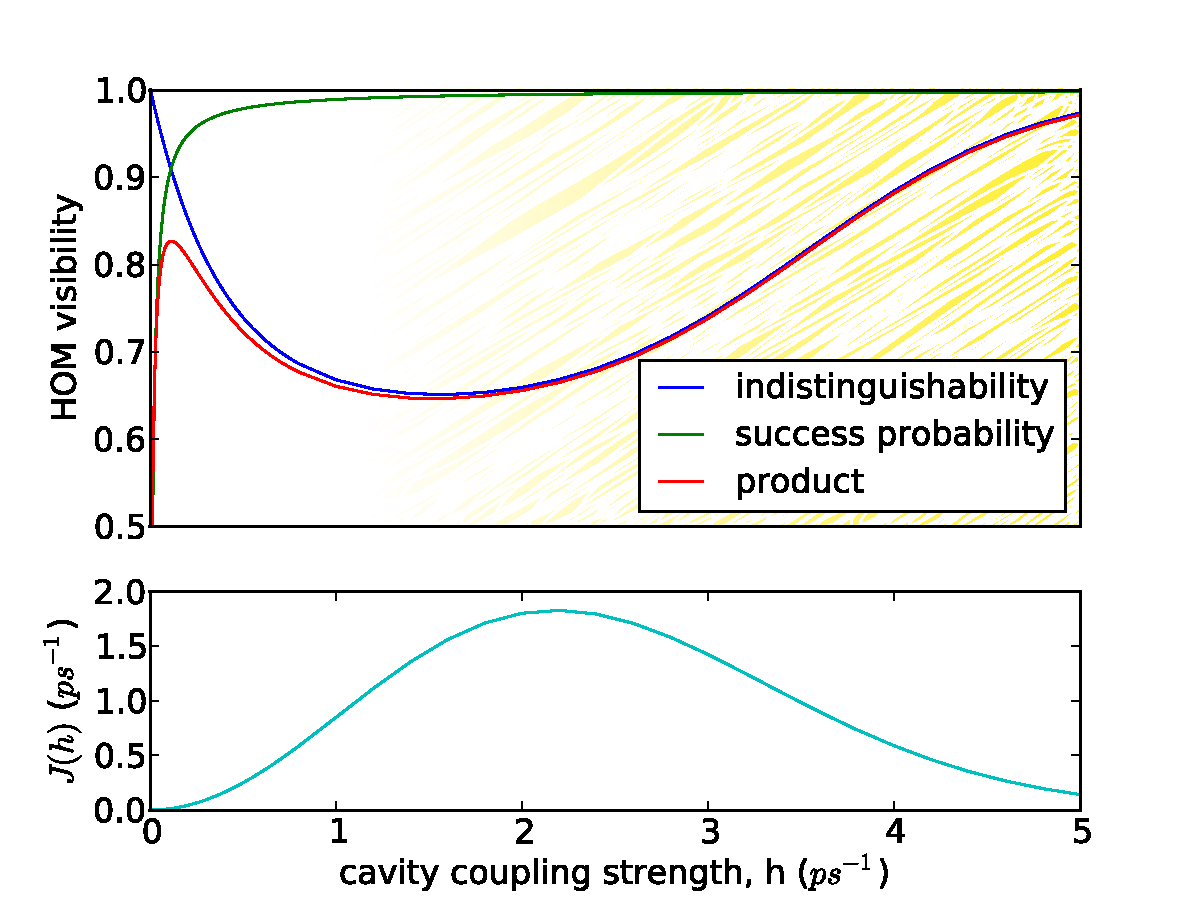
\includegraphics[width=12cm]{assets/2LS_plot.pdf}
  \end{center}
  \caption{Pulse-relax technique: calculations are performed as a function of the cavity coupling strength. Upper panel: at realistic coupling strengths ($h<1$) increased HOM indistinguishability necessarily entails a decrease in efficiency (success probability), with the product of the two (blue curve) approaching zero. Here the spontaneous emission rate is $\Gamma = 0.005~\mathrm{ps}^{-1}$. For overcoming phonon-induced decoherence and achieving a  high success probability, we must move into a region of unrealistically high $h$, represented by the increasing level of shading of this plot.
 The lower panel shows the phonon spectral density, Eq.~\ref{eq:specdens}, evaluated at the cavity coupling strength $h$, giving a rate that is directly proportional to phonon-induced dephasing during the pulse-relax process.
 }
  \label{2LS_plot}
\end{figure}

Fig.~\ref{2LS_plot} shows the HOM visibility obtained from, and spectral density used in, simulations of the pulse-relax technique. At low coupling strengths the phonon spectral density is small, and so phonon decoherence is largely avoided giving high indistinguishability. As described earlier, we have fixed $\kappa$, the cavity leakage rate, to be $3 h$ so the effective coupling to the the target mode is proportional to the Purcell factor $h^2/\kappa \sim h$. This means that, for small $h$, the rate of photon emission into the cavity mode is slow and thus spontaneous emission into environmental optical modes is a problem. To take account of this effect, we define the `combined HOM visibility', which is the product of success probability and bare HOM visibility, which approaches zero as $h \to 0$. Taking large coupling strengths allows one to access the region to the higher frequency side of the hump in the phonon spectral density and so could avoid this problem, but is unrealistic given the cavity parameters currently obtainable experimentally. In the experimentally feasible region ($h<1$)~\cite{vuckovic:12} we must therefore trade indistinguishability for efficiency.

\begin{figure}[htb]
  \begin{center}
  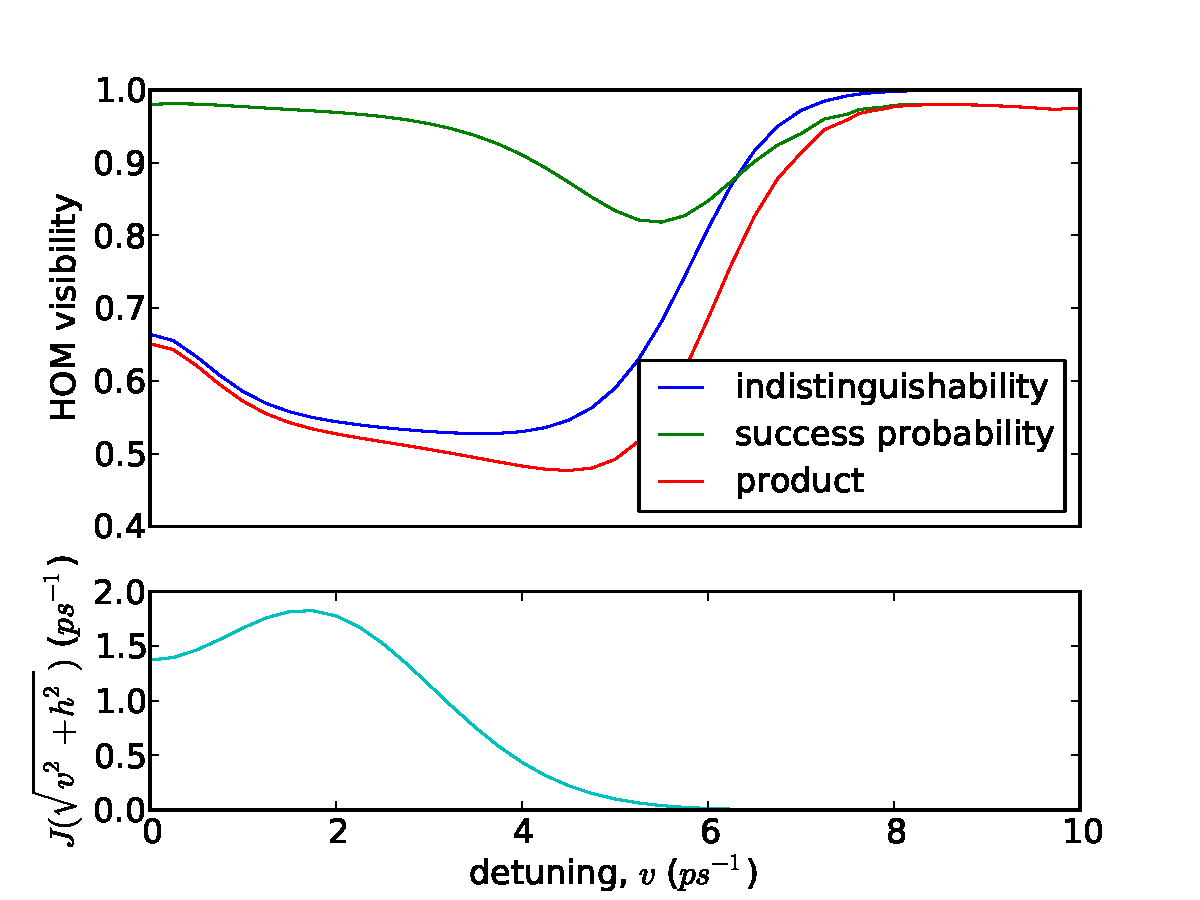
\includegraphics[width=12cm]{assets/raman_plot.pdf}
  \end{center}
  \caption{Raman technique, $h = 0.5$: by choosing a detuning to move beyond the region of high phonon spectral density we can achieve near-perfect indistinguishability. The efficiency in this region is high enough for a feasible photon source.}
  \label{raman_plot}
\end{figure}

In contrast, the Raman procedure (Fig.~\ref{raman_plot}) avoids this trade-off. For small detuning the visibility is low, but this is because we do not get a proper Raman ground state transition unless $\nu \gg h$. If this condition is not met, the system simply undergoes a non-optimal detuned pulse-relax transition. Once we reach a detuning of around $\nu = 12h (= 6~\mathrm{ps}^{-1})$ the indistinguishability and efficiency both  increase. Our choice of detuning size is limited in that it must be small in comparison with the original energy gap between the ground and excited states, and that it avoids any nearby excited states. This leaves us some freedom to use large detunings to push to frequencies above the region of high phonon spectral density. As the detuning is increased the efficiency saturates below unity. In this region both the time taken for the Raman process and the average excited state lifetime scale with the detuning squared, the two effects cancelling one another.

\begin{figure}[htb]
  \begin{center}
  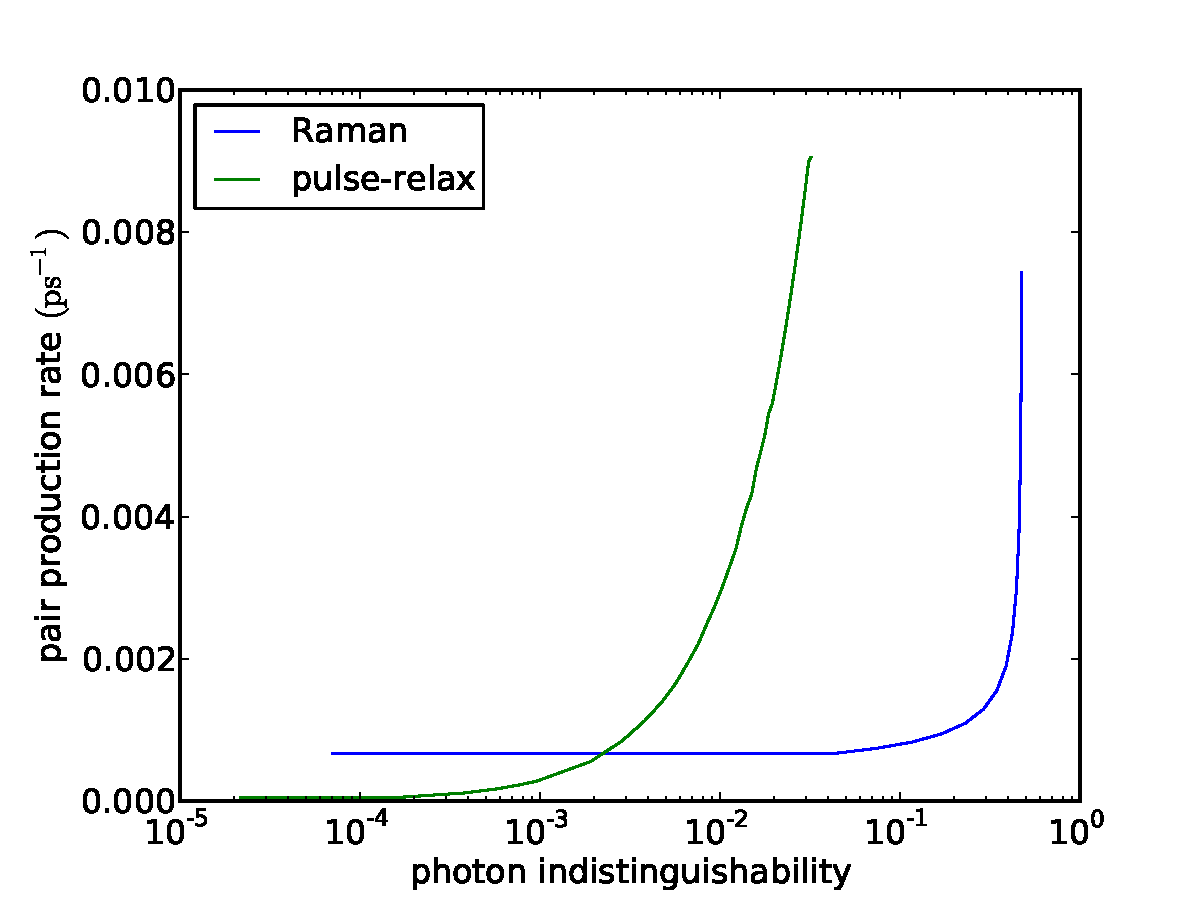
\includegraphics[width=12cm]{assets/no_spont_prod_rate.pdf}
  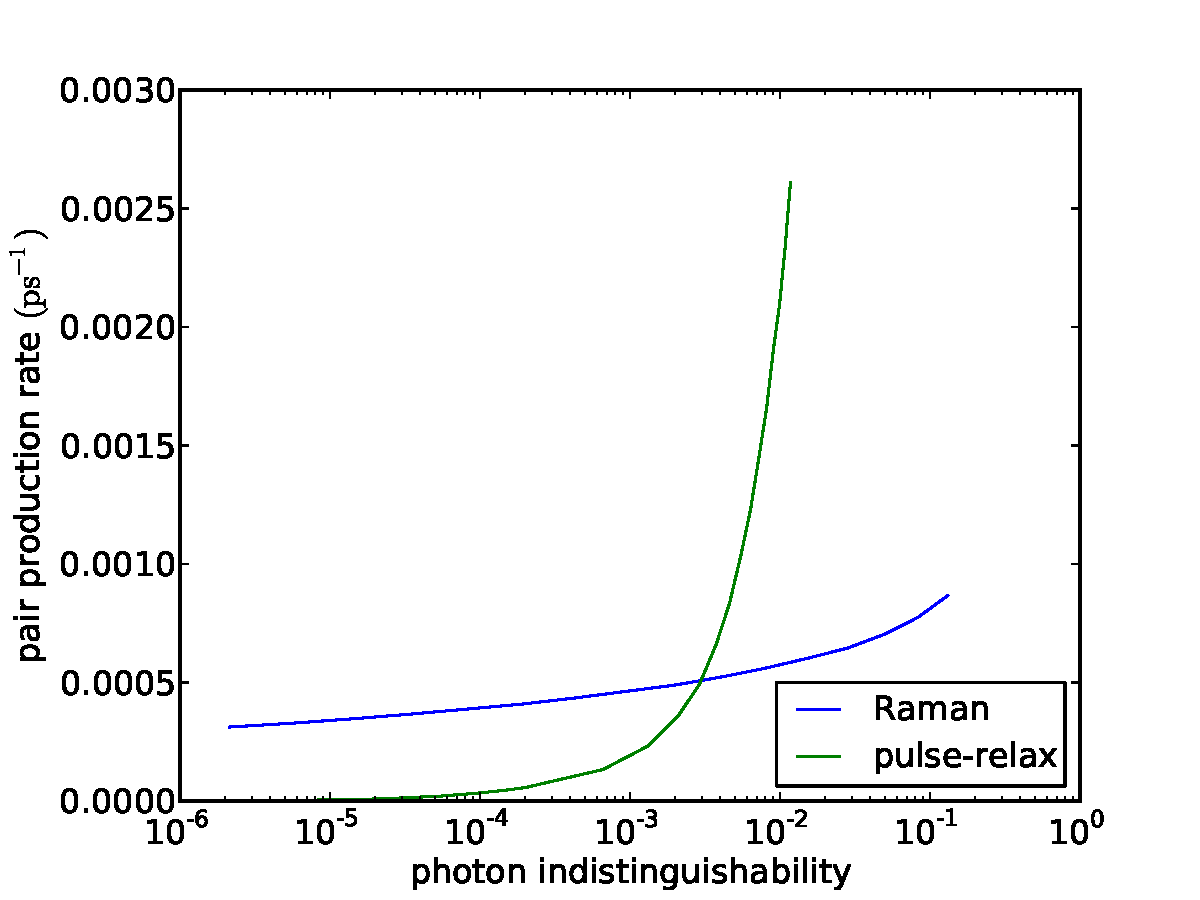
\includegraphics[width=12cm]{assets/rate_of_production_plot.pdf}
  \end{center}
  \caption{Rate of photon pair production: with no spontaneous emission (upper), and spontaneous emission with an excited-state lifetime of $200$~ps (lower)}
  \label{rate_of_production_plot}
\end{figure}

In many applications where photons are used, the product of efficiency and indistinguishability may not be the most useful metric for characterising the performance of the source; often photon escape errors can be accounted for, and the indistinguishability of photons that are detected is the important figure of merit. We therefore also calculate the rate of production of pairs of photons of a given indistinguishability using each approach (Fig.~\ref{rate_of_production_plot}). For our production rate we take
\begin{eqnarray}
  r_f = \frac{e_f}{t_f}
\end{eqnarray}
where $e_f$ is the efficiency and $t_f$ is the time taken for $99\%$ of the runs to have completed (possibly unsuccessfully), for parameters ($h$ in the pulse-relax scheme, and $\nu$ in the Raman scheme) chosen to obtain a given indistinguishability, $f$. This figure is somewhat approximate as it takes no account of how successful runs (where two photons are emitted into the correct modes) and unsuccessful runs are distributed within the process run time, and no allowance is made for time taken to reset the system in the event of a failure. The effect of the former is minor since in our model spontaneous emission can occur uniformly at any point of the process. We will revisit the effect of the latter shortly.

Even in the absence of spontaneous emission (Fig.~\ref{rate_of_production_plot}, upper panel), the Raman procedure is quicker than the pulse-relax process at generating photons of a sufficiently high level of indistinguishability. With the dephasing parameters chosen in our model this occurs for indistinguishability of greater than $99.9\%$. In our model, spontaneous emission is the only process degrading the efficiency -- without it we have perfect efficiency and so neither of the potential shortcomings discussed in the previous paragraph apply.

When spontaneous emission is added, we see a similar pattern but the indistinguishability threshold is very slightly lower. This is an upper bound, as here the reset time becomes important. The efficiency of the Raman procedure remains fixed at about $80\%$, requiring on average $1.25$ runs per pair. In contrast, the efficiency of the pulse-relax procedure heads towards zero, meaning that many attempts will be needed to produce a pair. If the time taken to reset the system (to the excited state $\ket{e}$ in which we have assumed the pulse-relax system starts) is large, the Raman procedure will become advantageous at a far lower threshold.

\section{Conclusion}

To conclude, we have developed a realistic and microscopically justified model of the impact of phonons on solid state single photon sources. We used a modified, `semi-quantum', master equation method for the efficient calculation of coincidence rates, without having to resort to a quantum Monte-Carlo simulation approach.

Our physical results are best summarised by considering the following scenario: suppose you are working with a system where phonon dephasing and spontaneous emission are the dominant loss channels, where you have some control over the cavity parameters ($h$ and $\kappa$), and that you are tasked with building a high indistinguisability, efficient, on-demand photon source. In this scenario, we find that a Raman technique is preferable to the pulse-relax approach. In particular, in addition to producing superior production rates at a given indistiguishability, the Raman approach we have taken only requires varying of the detuning - by tuning the cavity mode, and driving field - whilst leaving the other cavity properties fixed. This is in contrast in to the pulse-relax approach that we used for comparison where we allowed the cavity coupling strength itself to be varied within a realistic range of values. 




\chapter{The Power of Small Toric Codes} 
\label{ch:SurfaceCodes}

\section{Introduction to the Toric Code}

The ability to correct and recover from errors is important for any quantum computing scheme. The discovery of the first error correcting quantum codes by Shor in 1995 was vital for demonstrating that quantum computing was theoretically viable. The toric code is an error correcting code proposed by Kitaev \cite{kitaev_1, kitaev_2}, arising from work using quantum mechanics to provide simple models of topological order. It is the simplest and most elegant in the class of such codes, collectively known as surface codes \cite{kitaev_bravyi, planar_codes_freedman_meyer}.

One of the key advantages of surface codes is their local nature - the codes can be implemented on a two-dimensional lattice using only nearest neighbour interactions. In this realistic experimental scenario, surface codes can tolerate per-operation error rates of up to 1\% \cite{fowler11, fowler_classical_processing}, compared with rates in of the order of $10^{-4}$ for the early error correcting codes \cite{steane_code_shit}.

In this chapter we look towards an experimental realisation of the toric code and study the code for small values of $n$. We pre-compute a decoding library, an approach that quickly becomes intractible for values of $n$ above those considered here, but has the advantage that we obtain a provably optimum decoding success rate. We use our pre-computed decoder to assess the \textit{encoding power} of the code: we say the code has positive encoding power if the encoded qubits exhibit a lower error rate than the same number of unencoded qubits subjected to the same noise.

\section{Shor's Code Revisited}

Before moving on to the toric code, we first look at a simple example of an error correcting code in order to introduce some of the notation and concepts that we use later. For this purpose we pick the first stage of Shor's code \cite{shor_codes_95}. The full code uses nine qubits to protect against general errors; the code we analyse here uses only three qubits and protects only against a single error channel. We describe the code by specifying how to encode a general qubit:
\begin{align}\label{shor_state}
  \alpha\ket{0} + \beta\ket{1} \rightarrow \alpha\ket{000} + \beta\ket{111}.
\end{align}
The idea here is very simple: each logical qubit is encoded into three physical qubits. Shor constructed a circuit such that if there was a bit-flip error on any one of the three qubits, the state would automatically be corrected. The system basically implements a `majority vote' error correction scheme.

We now analyse this system in a different way, which will directly translate to our treatment of the toric code later in the chapter. In order to do this we first introduce the standard qubit operators:
\begin{align}
  Z &= \ket{0}\bra{0} - \ket{1}\bra{1} \\
  X &= \ket{0}\bra{1} + \ket{1}\bra{0} \\
  Y &= \ket{0}\bra{1} - \ket{1}\bra{0} = ZX.
\end{align}
In what follows we will need to apply these operators to states of multiple qubits. To do this we will introduce subscripts to the operators, so that, for example, $Z_1$ is the $Z$ operator acting on the first qubit. Operators acting on different qubits can be seen to commute with one another.

\begin{figure}\label{ops_states}
  \begin{center}
    \begin{tabular}{c c c c c}
      State & $Z_1 Z_2$ & $Z_2 Z_3$ & $Z_1 Z_3$ & $Z_1$ \\
      \hline
      $\ket{000}$ & $+1$ & $+1$ & $+1$ & $+1$ \\
      $\ket{001}$ & $+1$ & $-1$ & $-1$ & $+1$ \\
      $\ket{010}$ & $-1$ & $-1$ & $+1$ & $+1$ \\
      $\ket{100}$ & $-1$ & $+1$ & $-1$ & $-1$ \\
      $\ket{110}$ & $+1$ & $-1$ & $-1$ & $-1$ \\
      $\ket{101}$ & $-1$ & $-1$ & $+1$ & $-1$ \\
      $\ket{011}$ & $-1$ & $+1$ & $-1$ & $+1$ \\
      $\ket{111}$ & $+1$ & $+1$ & $+1$ & $-1$
    \end{tabular}
  \end{center}
  \caption{The eigenvalues of the operators on their simultaneous eigenstates}
\end{figure}

We will start by considering a state of three qubits and the set of operators $S = \{Z_1Z_2, Z_2Z_3, Z_1Z_3\}$. As these operators commute with one another it is possible to find states that are simultaneous eigenstates of all three. For the set $S$ that we have chosen we can take these to be the standard basis elements as shown in Fig. \ref{ops_states}. The operators we have chosen are not actually independent as
\begin{align}
  (Z_1Z_2)(Z_2Z_3) = Z_1Z_3.
\end{align}
The eigenvalue of the third operator can be inferred from the other two. To break the degeneracy in the eigenstates we introduce a fourth operator $Z_1$ that commutes with the elements of $S$.

We say that the set $T = \{Z_1Z_2, Z_2Z_3, Z_1\}$ is an \textit{independent} set of commuting operators. The eigenvalues of these operators uniquely define the basis states. We say that the set $T$ \textit{stabilises} the state $\ket{000}$, as $t\ket{000} = \ket{000}$ for all $t\in T$. Similarly $\{Z_1Z_2, -Z_2Z_3, Z_1\}$ stabilises $\ket{001}$. We call $T$ the \textit{stabiliser representation} of the state $\ket{000}$; by specifying three independent, binary-outcome operators in a Hilbert space of dimension $2^3$ we have uniquely defined the state.

We can also use the stabiliser representation to define a subspace of the Hilbert space. The set $\{Z_1Z_2, Z_2Z_3\}$ uniquely defines a subspace spanned by the states $\{\ket{000}, \ket{111}\}$, which is precisely the codespace defined in Eqn. (\ref{shor_state}). If we were to perform measurements corresponding to the operators $Z_1Z_2$ and $Z_2Z_3$ on our encoded state we would expect the outcome $+1$ in both cases, no matter how many times the measurement was repeated. We can consider a measurement of the operator $Z_1$ as a measurement of the encoded logical qubit.

Following Shor's approach, we model the introduction of errors as the $X$ and $Z$ operations acting on one or more of the qubits. To take a concrete example consider the error represented by $X_1$ acting on the state:
\begin{align}
  X_1 (\alpha\ket{000} + \beta\ket{111}) = \alpha\ket{100} + \beta\ket{011}.
\end{align}
If we evaluate the stabilisers now we find $Z_1Z_2 \rightarrow -1$ and $Z_2 Z_3 \rightarrow +1$. We can see from the stabiliser outcomes that we are no longer in the codespace and that an error has occurred. You will notice that the error was visible only in the outcome of the stabiliser that anti-commuted with the error operator: $(Z_1Z_2)X_1 = -X_1(Z_1Z_2)$.

Although we can tell that an error occurred, we do not know if it was $X_1$ or $X_2X_3$. In Shor's scheme we correct the most likely. A different way of looking at this is that we can return to the codespace by applying $X_1$: if the error was actually $X_1$, the logical qubit will be intact, but if the error was $X_2X_3$ the overall operation will be $X_1X_2X_3$ and there will be an error on the logical qubit.

If we instead have a phase flip $Z_1$ we will not be able to detect the error, as $Z_1$ commutes with all the stabilisers and will go unseen. In Shor's original paper he fixes this by expanding the codespace.

We have introduced the stabiliser notation to describe a familiar code and have seen how by measuring stabiliser operators we can detect certain errors. We have an operator that completes the commuting set that defines an operation on the logical qubit and that we can detect errors provided they do not commute with all of the stabilisers. We will now use this language to introduce the toric code.

\section{Definition of Toric Codespace}

The toric $2n$-code (Fig. \ref{4-code}) uses $2n^2$ physical qubits to encode two logical qubits. The codespace is most elegantly described using the stabiliser formalism. In particular we shall specify a set of $2n - 2$ independent stabilisers to give a codespace of dimension four.

To describe the code, it is useful to picture the $2n^2$ physical qubits positioned on the odd diagonals of a $2n \times 2n$ lattice (i.e. in the positions with coordinates $(i,j)$, where $i+j$ is odd). On the sites $(i, j)$ where $i$ and $j$ are both even we construct an \textit{X-stabiliser}, $s^X_{k}$, by taking the product of $X$ operators of qubits on the neighbouring squares. When considering what we mean by `neighbouring' we identify opposite edges of the lattice, hence the `toric' nature of the code. On the sites $(i,j)$ where $i$ and $j$ are both odd, we define the \textit{Z-stabilisers}, $s^Z_{k}$, in a similar manner.
\begin{figure}[htb]
  \begin{center}
    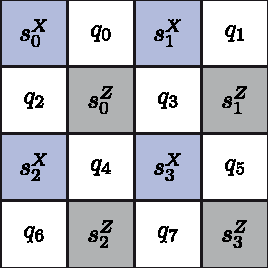
\includegraphics[width=5cm]{assets/4-code.pdf}
  \end{center}
  \caption{Qubit lattice for the $4$-code. $s_{k}^X$ and $s_{k}^Z$ are $X$- and $Z$-stabilisers represented by the sites respectively. $q_i$ are qubits. By way of example, $s_{0}^X = X_0 X_2 X_1 X_6$ and $s_{0}^Z = Z_3 Z_4 Z_2 Z_0$.}
  \label{4-code}
\end{figure}

We let $S_X = \{s^X_{k}\}$. There are $n^2$ elements in $S_X$, but only $n^2-1$ independent elements, as the final element is the product of all the others. We similarly define $S_Z = \{s^Z_{k}\}$. We will later use the sets $S_X$ and $S_Z$ to define the stabilisers of the codespace. Practically we will make measurements of these operators to check whether our state is still in the codespace. 

Just as in Shor's code, to fully define a state we will need to add additional commuting operators to our set of stabilisers. We now construct a set of operators that will be used for this purpose. We define $X_h$ (horizontal X) to be the product of $X_i$s acting on qubits in an even row, $X_v$ (vertical X) the product of $X_i$s acting on qubits in an even column, and similarly, $Z_h$ to be $Z_i$s on an odd row, and $Z_v$ to be $Z_i$s on an odd column. Any of the pairs $\{X_v, X_h\}$, $\{X_v, Z_v\}$, $\{Z_v, Z_h\}$, and $\{Z_h, X_h\}$ will suffice to fully define the state. The remaining pairs, $\{X_v, Z_h\}$ and $\{X_h, Z_v\}$, satisfy the standard qubit commutation relation, $[X, Z] = 2iY$, and so we can use this set of \textit{logical operators}, $L = \{X_v, X_h, Z_v , Z_h\}$, to define a pair of independent \textit{logical qubits}. 

We will now turn to how errors are detected in the toric code. As with the treatment of the Shor code we will consider an error to be a set of individual $X$ and $Z$ errors applied to a subset of the physical qubits. An $X$-error on a single qubit will flip the eigenvalue of the neighbouring $Z$-stabilisers, but commutes with the $X$-stabilisers and will not be detected by them. Similarly, a $Z$ error will be detected by the $X$-stabilisers and not the $Z$-stabilisers, and a $Y$ will be detected by both sets. Additional errors will cause the stabiliser eigenvalues to toggle. If errors occur sequentially they will be detected by the stabilisers at either end of the chain.


\begin{figure}[htb]
  \begin{center}
    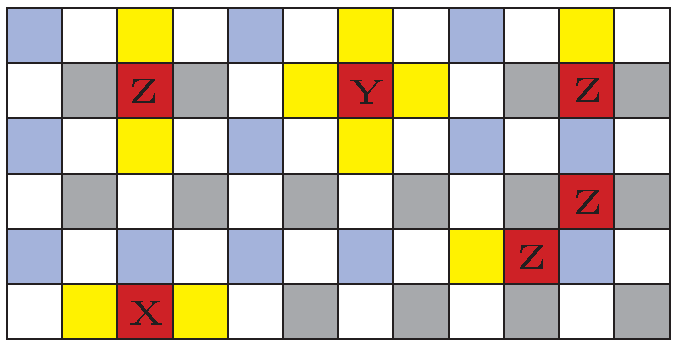
\includegraphics{assets/basic_errors.pdf}
  \end{center}
  \caption{Error detection of isolated $Z$-, $X$-, $Y-$errors and a chain of $Z$-errors.}
  \label{basic_errors}
\end{figure}

\section{Code Variants}

In the rest of the chapter, we will consider three variants of the toric code, that we refer to as the \textit{classical toric code}, the \textit{reduced quantum toric code} and the \textit{full quantum toric code}.

\subsection{Classical Toric Code}

In the classical toric code we completely ignore the phase of each qubit, concerning ourselves only with the outcomes of measurements on the logical qubits in the $Z$-basis. To define the codespace we take our set of code stabilisers $S$ to be the set $S_Z$ and the set of logical operators $L=\{Z_h, Z_v\}$. The codespace is massively degenerate but any state in it will be sufficient for our purposes.

We simplify the analysis by considering only $X_i$ errors on the individual qubits, as these are the only ones that can affect the measurement outcomes we are interested in. We define the complete set of error operators, $E$, to be the set generated by the individual qubit $X_i$ operators - that is the set of all products of such operators. As the $2n^2$ individual qubit operators, $X_i$, commute with one another and as $X_i^2 = \id$ we can show that $|E| = 2^{2n^2}$.

We also introduce the set of \textit{syndromes}, $A$ - the possible outcomes when the code stabilisers $S$ are measured. When each stabiliser measurement outcome is $+1$ we say we have obtained the \textit{zero-syndrome}, which we denote by the element $a_0 \in A$. If we obtain the zero-syndrome we know that we are in the codespace. In the classical toric code we have that $|A| = 2^{n^2-1}$, as each of the $n^2$ elements of $S$ can report $\pm 1$, but the last outcome is fixed by the others.

\subsection{Full Quantum Toric Code}

For the full quantum toric code, we aim to fully protect our encoded qubits against all sources of error. We take a full set of code stabilisers, $S = S_X \cup S_Z$, and the full set of logical operators $L = \{Z_h, Z_v, X_h, X_v\}$. The complete set of errors is generated by the set of all individual qubit operators $\{X_i, Z_i\}$, so that $|E| = 4^{2n^2}$.

Following similar reasoning to the classical toric code we can deduce the size of the set of syndromes, $A$: the outcomes of each of the $2n^2 - 2$ independent stabilisers in $S$ completely define a syndrome, so that $|A| = 2^{2n^2-2}$.

\subsection{Reduced Quantum Toric Code}

The reduced quantum toric code is slightly more subtle that the previous two cases. We take the full set of stabilisers $S = S_X \cup S_Z$ and logical operators $L = \{Z_h, Z_v, X_h, X_v\}$, but aim only to protect against individual qubit $Y_i$ errors. As previously, it is straightforward to show that $|E| = 2^{2n^2}$. It is more difficult to determine the size of $A$ in this case, as not all syndromes are possible from the errors that we consider. It is possible to show that $|A| = 2^{2n(n-1)}$.

\section{The Structure of the Code}

We now investigate the structure of the set of errors, $E$, and how they relate to the syndromes, $A$, and logical errors, $L$. We begin by defining the function
\begin{align}
  \text{synd}: E \rightarrow A
\end{align}
that maps an error onto its associated syndrome. We are then able to define
\begin{align}
  E_a = \{ e\in E : \text{synd}(e) = a \},
\end{align}
the set of all possible errors corresponding to a syndrome $a$. For convenience we define $E_0 = E_{a_0}$ to be the set of errors corresponding to the zero-syndrome, $a_0$. If an error in $E_0$ occurs it will go undetected by the code. We define a function to act on the set $E_0$,
\begin{align}
  \text{lerr}: E_0 \rightarrow L,
\end{align}
taking an error to the corresponding logical error on the encoded qubits. Finally we define the set
\begin{align}
  E_{0, l} = \{ e\in E_0: \text{lerr}(e) = l \}.
\end{align}
It is easy to see that each $E_{0, l}$ contains at least one element, as $l$ itself is a member: by applying a set of errors corresponding to a logical operator, we apply this operator to the encoded qubits, inducing a logical error.  We will now show that the sets $E_{0,l}$ have exactly the same number of elements - our first important result about the structure of our toric codes.


\begin{figure}[htb]
  \begin{center}
    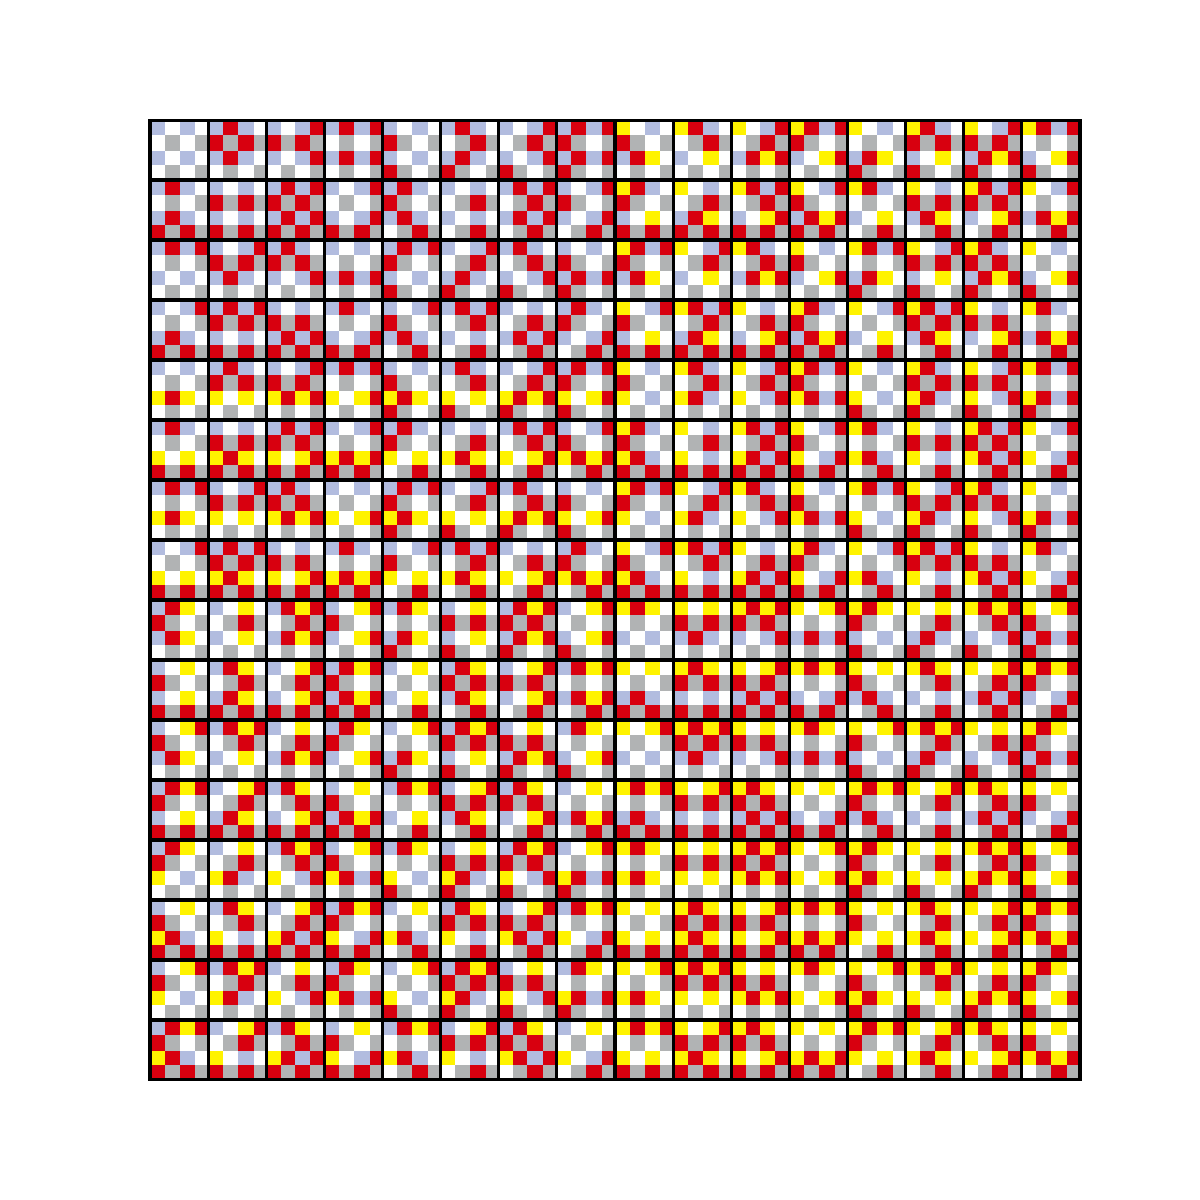
\includegraphics{figures/4_array.pdf}
  \end{center}
  \caption{Full set of errors, $E$, for the classical $4$-code.}
  \label{4_array}
\end{figure}

To show that the $E_{0, l}$ are all the same size, we will show that they all have the same number of elements as $E_{0,0}$ - the set of elements of $E_0$ that introduce no logical error. To see this, take element $e_1 \in E_{0, l}$ and $e_2 \in E_0$. We claim that
\begin{align}
  e_2 \in E_{0, l} \Leftrightarrow e_1 e_2 \in E_{0,0}.
\end{align}
The proof of the claim follows from the fact that all logical operators $l\in L$ are products of individual qubit operators, so that $l^2 = \id$: by applying the same logical error twice we undo it. If by applying $e_1$ after $e_2$ we have no logical error, they must be in the same error class, and the converse is also true. We now consider the set
\begin{align}
  e_1 E_{0,0} = \{e_1 e : e \in E_{0,0}\}
\end{align}
and claim that, given $e_1 \in E_{0,l}$, we must have $E_{0, l} = e_1 E_{0,0}$. This follows as, 
\begin{align}
  e_2 =  e_1 e \Leftrightarrow e_1 e_2 = e,
\end{align}
where we have used that $e_1^2 = \id$. Therefore we can use $e_1$ to establish a bijection between $E_{0,l}$ and $E_{0,0}$ and so the sets must have the same number of elements.

We now move on to the sets of errors, $E_a$, corresponding to a general syndrome, $a \in A$. As we have taken $A$ to be the set of obtainable sydromes, it follows that there must be at least one element in each set $E_a$. It is useful to assume that we have chosen an arbitrary member from $E_a$. We call this a \textit{matching} for the syndrome, and denote our specific choice of matching $m^*(a)$. In practice there are many ways to construct a specific matching for each syndrome $a$, for example see Fig.~\ref{matching}. If we observe the syndrome $a$ and apply the matching $m^*(a)$ we are guaranteed to be back in the codespace.

\begin{figure}[htb]
  \begin{center}
    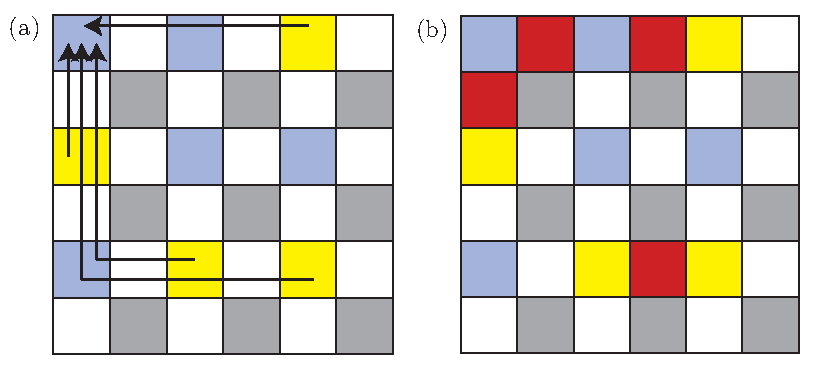
\includegraphics{figures/matching.pdf}
  \end{center}
  \caption{Constructing a specific matching for a classic code: the detected errors are first moved to the left, then to the top, of the lattice (a); we apply a $Z$ operator to any qubit that has been passed over an odd number of times (b).}
  \label{matching}
\end{figure}

Following a similar procedure to before we can show that $E_a = m^*(a) E_0$, and therefore each of the sets $E_a$ have the same number of elements. Furthermore we can split the set $E_a$ up into a set of classes
\begin{align}
  E_{a,l} = m^*(a) E_{0, l}.
\end{align}
The set $E_{a,l}$ can be interpreted as the set of errors that when corrected by $m^*(a)$ induce the logical error $l$ on the encoded qubits. All the sets $E_{a, l}$ have the same number of elements as $E_{0,0}$.

In the preceding paragraphs we have split up the total set of errors $E$ into identically sized subsets $E_{a, l}$ indexed by $a\in A$ and $l\in L$. It follows immediately that
\begin{align}
  |E| = |A| \cdot |L| \cdot |E_{0,0}|.
\end{align}
You can see that this relationship holds for our three code variations in Fig.~\ref{code_sizes}.

\begin{figure}\label{code_sizes}
  \begin{center}
    \begin{tabular}{c c c c c}
      Code & $|E|$ & $|A|$ & $|L|$ & $E_{0,0}$ \\[1.5ex]
      \hline \\[0ex]
      Classical         & $2^{2n^2}$ & $2^{n^2-2}$ &  4 & $2^{n^2-2}$ \\[3ex]
      Reduced Quantum   & $2^{2n^2}$ & $2^{2n(n-1)}$ &  4 & $2^{2n-2}$ \\[3ex] 
      Full Quantum      & $4^{2n^2}$ & $2^{2n^2-2}$ & 16 & $2^{2n^2-2}$
    \end{tabular}
  \end{center}
  \caption{Sizes of the sets involved with our three toric code variants.}
\end{figure}

We have shown that given a syndrome always corresponds to multiple logical error classes, of which we can correct only one. We still have to answer the question of which one to correct. In the Shor code case we picked the matching to minimise the probability of introducing a logical error. Ideally that is what we would do here too. This of course depends on the error model, which we have not discussed yet. It is also not straightforward to do. The number of matchings in each class grows exponentially with the size of the grid. No efficient way of calculating the probabilities is know, even for the simplest error model.

The job of picking a matching given a syndrome falls to a decoder. These are often heuristic procedures, designed to balance calculation time with identifying the most likely class as often as possible. Determining a good decoding strategy is currently a very active area of research and there are a number of different approaches \cite{poulin_renormalisation, fowler_classical_processing, wooton_mcmc1}. It is not only important that a decoder maximises the probability of returning to the codespace without inducing an error on the logical qubits, but also that the decoder can run in a reasonable amount of time. 


%\subsection{Existing Decoding Strategies}

%Determining a good decoding strategy is currently a very active area of research. It is not only important that a decoder maximises the probability of returning to the codespace without inducing an error on the logical qubits, but also that the decoder can run in a reasonable amount of time. Here we look at three leading decoding strategies: minimum weight path matching, renormalisation, and Markov chain Monte Carlo.

%Minimum weight path matching (MWPM) aims to minimise a cost associated with the matching. The first stage of the algorithm is to take the firing stabiliser sites and place them on the nodes of a graph. An edge is then constructed between each pair of nodes with a weight representing the cost of connecting the sites on the lattice. A common choice is to take the Manhatten distance between the nodes, but it is possible to construct different weights to take addition information into account such as inhomogeneous error rates. Edmond's minimum weight path matching algorithm is then run on the graph, to pair up all the nodes whilst minimising the total weight of the edges chosen. This procedure is run separately on the $X$- and $Z$-syndromes, but it is possible to modify the procedure to take into account correlations between the syndromes caused by $Y$ errors.

%MWPM is $O(n^2)$ in the length of the lattice \cite{fowler11}. It provides good results especially in the low error case, when the minimum weight matching has a high probability of belonging to the most likely error class. Conceptually it is a little unsatisfactory that the algorithm is not truly aiming to find the most likely error class. The other two strategies have been shown to outperform MWPM in the case of high error rates, but this point is somewhat moot as it is unlikely that a quantum computer would function in this regime. A more troubling feature is that there is no natural way to incorporate additional classical information that may be available from the experimental procedure beyond altering the edge weights in an ad.\ hoc.\ fashion.

%The renormalisation approach involves splitting the lattice into sublattices, producing a matching on the sublattices and then combining the results to produce a matching for the complete lattice. The approach is recursive, in that the same procedure is applied to each sublattice. 

%The Markov chain Monte Carlo method aims to estimate the probabilities of each of the error classes consistent with the observed syndromes, by randomly sampling from each class using the Manhatten algorithm. 


\section{Error Model}

We consider depolarising noise distributed uniformly over the lattice with a given, constant probability:
\begin{equation} \label{noise_eq}
  D(\rho) = p_x X\rho X +  p_z Z\rho Z + p_y Y\rho Y  + (1- p_x - p_y - p_z)\rho.
\end{equation}
The values of $p_x$, $p_y$ and $p_z$ vary over our different code variants accordingly
\begin{enumerate}
  \item Classical case: $p_x = p$, $p_y = p_z = 0$
  \item Reduced quantum case: $p_y = p$, $p_x = p_z = 0$
  \item Full quantum case: $p_x = p_y = p_z = p/3$.
\end{enumerate}

We also consider the effect of stabiliser sites mis-reporting the stabiliser measurement outcomes: that with some probability, $q$, the stabiliser reports that it fired (/did not fire) when it did not (/did). The normal approach here is to consider multiple faulty stabiliser evaluations as extending the code into a third dimension. By observing the stabiliser outcomes over multiple rounds it is possible to increase the chance of correctly identifying any mis-reported outcomes.

We just consider a single round of stabiliser evaluation, and so this extra information is not available to us. Instead we try to identify and correct the right syndrome based on the syndrome we see. Even in multi-round systems the final step will look like this and so our results are an upper bound on the possible decoding probabilities for small systems.

\section{A Precomputed Decoder}

We begin by looking at the probability of getting a particular logical error, $l$, given that syndrome, $a$, occurs and we attempt to correct it using our chosen matching method by applying $m^*(a)$:
\begin{align}
  p(l \vert a) = \sum_{e \in E_{a,l}} \frac{p(e)}{p(a)}. 
\end{align}
For each stabiliser outcome $a$ we identify the most likely logical error $l_a$, such that $p(l_a \vert a)$ obtains a maximum. In cases where the most likely logical error is not unique we pick arbitrarily between the candidates. We may then correct our ealier attempt by applying the operator $l_a$, so that the total correction operation on the state will be $l_am^*(a)$. The overall successful decoding probability from following this procedure is 
\begin{align}
  P_d &= \sum_{a \in A} p(l_a \vert a)p(a) \\
  &= \sum_{a \in A} \max_{l\in L} \left\{ \sum_{e \in E_a} \frac{p(e)}{p(a)} \right\} p(a) \\
  &= \sum_{a \in A} \max_{l\in L} \left\{ \sum_{e \in E_a} p(e) \right\}. \label{truthful_prob}
\end{align}

When considering mis-reported stabiliser outcomes we must relax the restriction that there will be an even number of firing stabiliser sites. We let $A'$ be the set of all possible stabiliser outcomes $A' = \{0, 1\}^{\otimes n^2}$. If we are to successfully decode a syndrome $a'$, we must first identify the correct syndrome $a$, on which to perform the arbitrary matching, and then identify the most likely logical error $l_a$ to correct. If we identify the wrong $a$, the final state will not even be in the code space. Given $a'$ we must pick $a$ and $l$ to provide the maximum probability of a successful decoding in the case of mis-reporting stabiliser outcomes:
\begin{align}
  P'_d &= \sum_{a' \in A'} p(\text{success} \vert a') p(a') \\
  &= \sum_{a'\in A'} \max_{a \in A} \left\{ p(l_a \vert a) p(a \vert a') \right\} p(a')\\
  &= \sum_{a'\in A'} \max_{a \in A} \left\{ \max_{l \in L} \left\{\sum_{e \in E_a} \frac{p(e)}{p(a)} \right\} p(a \cap a') \right\}\\
  &= \sum_{a'\in A'} \max_{a \in A} \left\{ \max_{l \in L} \left\{\sum_{e \in E_a} p(e) \right\} p(a' \vert a) \right\}. \label{lying_prob}
\end{align}
While equations (\ref{truthful_prob}) and (\ref{lying_prob}) are conceptually simple, calculations are beset by difficulties due to the rapid growth in the size of the sets $E_{a,l}$, $A$, and $A'$: in the single noise channel case for the $2n$-code $|E_{a,l}| = |A| = 2^{n^2-1}$; for the full noise channel $2n$-code $|E_{a,l}| = |A| = 2^{2n^2 - 2}$. For example, the total number of error configurations, $|E|$, for the $6$-code is $2^{36}$, which would require $\sim200$GB of storage space.

Thankfully, we do not need the complete set of error configurations to compute the value of $p_\text{success}$ in Eq.~(\ref{truthful_prob}). For each configuration $e\in E$ the probability is
\begin{align}
  p(e) = (1-p)^{2n^2 - n(e)} p^{n(e)}
\end{align}
where $n(e)$ counts the number of errors in error configuration $e \in E$. When summing over the errors consistent with a given logical error and syndrome we get
\begin{align}
  \sum_{e \in E_{a,l}} p(e) &= \sum_{e \in E_{a,l}} (1-p)^{2n^2 - n(e)} p^{n(e)} \\
  &= (1-p)^{n^2} \sum_{i = 0}^{2n^2} d_{a,l}^{(i)} \left(\frac{p}{1-p}\right)^i \\
  &=: (1-p)^{n^2} \chi_{a,l}\left(\frac{p}{1-p}\right)
\end{align}
where $d_{a,l}^{(i)} = \vert \left\{e \in E_{a,l} : n(e)=i \right\} \vert$ and we have used the final line to define the characteristic function $\chi_{a,l}$ of the class $E_{a,l}$. By computing and storing the coefficients $d_{a,l}$ we are able to calculate the success probabilities for a range of values of $p$.

The full source code used for our calculations, along with the computed tables of characteristic function coeffients, is available online \cite{toric_code_program}.

\section{Simulation Results}

\subsection{Classical Toric Code}

Using the method described, we calculated the success probabilities $P_d(n, p)$, and compared them with $p_{\text{bare}} = (1-p)^2$, the probability that two non-encoded qubits would remain error-free (Fig. \ref{x_results}).
\begin{figure}[htb]
  \begin{center}
    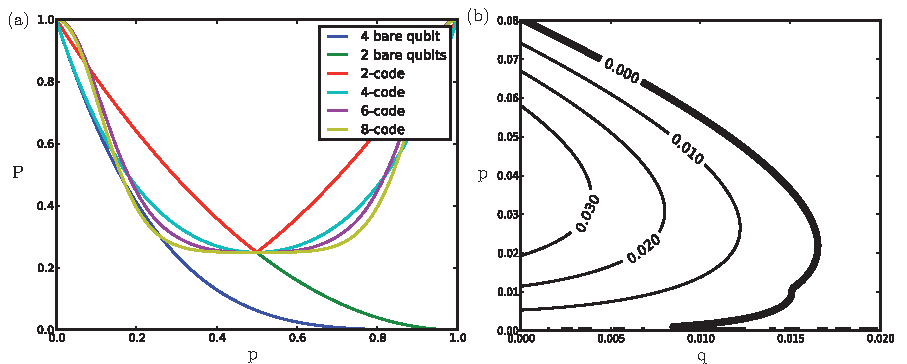
\includegraphics{figures/x_results.pdf}
  \end{center}
  \caption{Success probabilities for classical toric code: (a) shows the success probability, $P$, for ideal version of the code vs.\ the error rate, $p$, with two and four unprotected qubits for comparison; (b) shows the power of the $6$-code in the case when stabiliser outcomes are misreported with probability $q$.}
  \label{x_results}
\end{figure}

The $2$-code performs exactly the same as the bare qubits. This is not suprising, as the $2$-code has 2 physical code qubits and no error detect capacity - there is only one possible syndrome. The $4$-code performs worse than the bare qubits. Although the $4$-code has error-detect capacity, it has no error correct capacity. This can be seen by considering the case when a single error occurs - due to the translational symmetry of the lattice, the sydrome can give us no information about whether our correction introduced a logical error or not. For the $4$-code to be successful there must be no errors on the $4$ qubits that $X_h$ and $X_v$ measure, an event with probability approximately equal to $(1-p)^4$ for small $p$.

The $6$-code is the smallest code that exhibits encoding power for some values of $p$. Provided that $p < 0.1??$ the $6$-code outperforms the bare qubits. The $8$-code appears to offer roughly the same performance as the $6$-code. We weren't able to go beyond $2n=8$ with the computing resources available, but we expect that as $n$ increases the curves would tend towards a step function at the one-channel threshold.  We looked at the mis-reported stabiliser outcome case for the $6$-code. There is a small region with positive encoding power, that requires stabiliser fidelity in the region of $1\%$.

\subsection{Reduced Quantum Code}

For the reduced quantum code, we find that the $4$-code is the first code to offer encoding power in this scenario (Fig. \ref{y_results}). As before the $2$-code has no error detect capacity. Unlike before, the $4$-code is able to detect and correct errors, as it can use both $X$- and $Z$-stabiliser information to break the symmetry and pinpoint the error. 

We investigated the case of mis-reported stabiliser measurement outcomes for the $4$-code. We obtain positive encoding power for mis-reporting rates of up to 10\%. Overall the reduced quantum code shows remarkable encoding power, even for small codes. In using the full stabiliser information to detect a reduced set of errors, we have managed to hugely reduce the size of each error class (Fig.~\ref{code_sizes}). 
\begin{figure}[htb]
  \begin{center}
    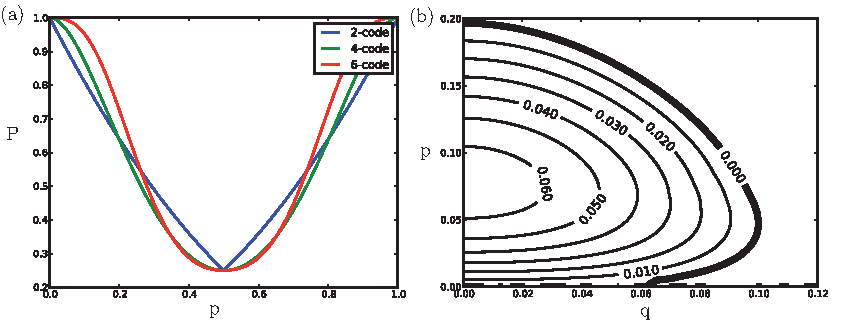
\includegraphics{assets/y_results.pdf}
  \end{center}
  \caption{Success probabilities for reduced quantum toric code: (a) shows the success probability, $P$, for ideal version of the code vs.\ the error rate, $p$, with two and four unprotected qubits for comparison; (b) shows the power of the $4$-code in the case when stabiliser outcomes are misreported with probability $q$.}
  \label{y_results}
\end{figure}

The circumstances that could justify the assumptions of the reduced quantum code are not unrealistic: we envisage a system with a single dominant error channel. In picking this to be the $Y$ channel, we exploit the lack of symmetry in our code effectively tayloring our code to be effective against the dominant error channel.

\subsection{Full Quantum Code}

Finally we look at the full code, protecting against full depolarizing noise, taking $p_x = p_y = p_z$ in equation (\ref{noise_eq}). 

\begin{figure}[htb]
  \begin{center}
    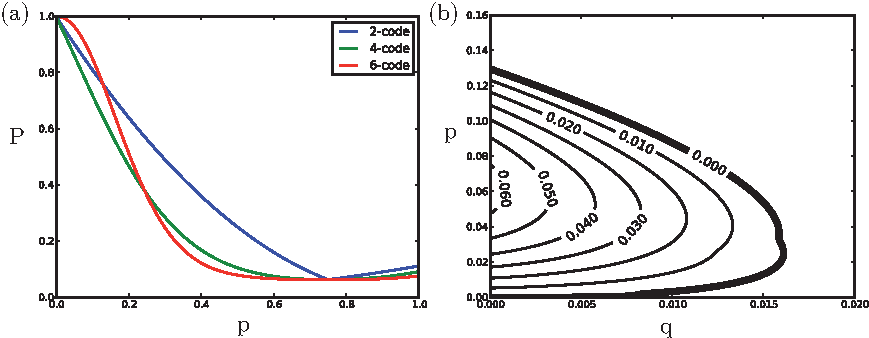
\includegraphics{assets/full_results.pdf}
  \end{center}
  \caption{Success probabilities for full quantum code: (a) shows the success probability, $P$, for ideal version of the code vs.\ the error rate, $p$, with two and four unprotected qubits for comparison. Note that the graph has a minimum at $p=0.75$ when the probability of each error is equal to the probability of no error. (b) shows the power of the $6$-code in the case when stabiliser outcomes are misreported with probability $q$.}
  \label{full_results}
\end{figure}

The $6$-code is the first code to offer encoding power (Fig. \ref{full_results}). We looked at mis-reported stabiliser outcomes for the $6$-code. Due to computational constraints we were only able to find a lower bound for $P'_d(p, q)$. This was obtained by modifying equation (\ref{lying_prob}) to maximise only over $a$ close to $a'$:
\begin{align} \label{approx_eq}
  p(\text{success})= \sum_{a'\in A'} \max_{a \in N(a',x)} \left\{ \max_{l \in L} \left\{\sum_{e \in E_{a,l}} p(e) \right\} p(a' \vert a) \right\}
\end{align}
where $N(a', x) = \left\{a \in A : d(a', a) \leq x \right\}$ with $d(a', a)$ the number of stabilisers where $a'$ differs from $a$. We took $x = 2$ to produce a rough region, and then used $x=4$ to refine the boundary. 

\section{An Experimental Suggestion}

Our aim in this section is to provide a criterion which an experimentalist can use to verify whether a given candidate toric code set-up is providing protection.

Our criterion is based on the observation that the $2$-code is essentially equivalent to two unprotected qubits: the sydrome outcome is always $+1$ so we are unable to even detect errors and the logical operations reduce to single qubit operations. By comparing the performance of the candidate code system against that of the $2$-code we are able to say whether the candidate system is exhibiting protective power. 

We do not specify the decoder that the experimentalist must use for the larger code (decoding is trivial in the $2$-code), but our precomputed decoder will give optimal results. In our analysis we assumed that the stabiliser mis-reporting and physical qubit errors are independent events. A round of stabilisers is permitted to introduce physical qubit errors, but these must be sprinkled evenly over the lattice and not be correlated with mis-reporting sites. If strong correlations were to exist a modified decoder would give a better chance of satisfying the criterion.

We assume that an experimentalist has the ability to perform all $X$- and $Z$-stabiliser measurement operations and the logical X measurements. In a large code the logical operations are potentially tricky, given their non-local nature. Here, due to the size of the codes considered, the logical operations actually involve fewer qubits than the stabilisers, and so are likely to be less technically demanding.

Our experimental proposal is as follows:
\begin{enumerate}
  \item Measure  $X_v$, $X_h$, and the stabilisers to find intitial syndrome $a'_i$ and logical qubit states $(x^v_i, x^h_i)$\label{first_step}
  \item Wait. Manually introduce noise if required.
  \item Measure $X_v$, $X_h$, and the stabilisers to find final syndrome $a'_f$ and logical qubit states $(x^v_f, x^h_f)$
  \item Decode the calculated syndrome, $a' = a'_i \text{\,XOR\,} a'_f$, to find matching $m$ \label{decode_step}
  \item Modify $(x^v_f, x^h_f)$ to reflect what the outcomes would have been if we had applied $m$ before measurement to find $(x^v_m, x^h_m)$
  \item If $(x^v_i, x^h_i) = (x^v_m, x^h_m)$ count the round as a success; if not, count the round as a failure.\label{last_step}
  \item Repeat steps \ref{first_step} to \ref{last_step} many times to calculate an experimental successful decoding probability $P_\text{d}^\text{expt}$
\end{enumerate}

We then repeat this procedure for the $2$-code and compare the results: if the larger system outperforms the $2$-code protection is provided. 


\section{Conclusion}

We have provided a protocol and pre-computed decoder for demostrating toric encoding size at minimal scale. The $2n$-code requires a minimum of $2n^2$ physical code qubits, plus an auxiliary qubit with which we must be able to perform CNOT operations with any of the code qubits. For the $4$-code this is a requirement of $9$ qubits and for the $6$-code the requirement is $19$ qubits. The error rates provided are not unrealistic for current experimental systems. 


%\clearpage
\singlespacing
%\addcontentsline{toc}{chapter}{Bibliography}
\bibliographystyle{cj}
\bibliography{/Users/tomclose/Documents/Quantum/tom_close}
\end{document}
